\documentclass[12pt,titlepage,ngerman]{article}

\usepackage[ngerman]{babel}
\usepackage[utf8]{inputenc}
\usepackage{color}
\usepackage[a4paper,lmargin={2,54cm},rmargin={2,54cm},tmargin={2.54cm},bmargin = {2.54cm}]{geometry}
\usepackage{enumitem}
\usepackage{amssymb}
\usepackage{amsthm}
\usepackage{graphicx}
\usepackage{acronym}
\usepackage[backend=bibtex,style=alphabetic]{biblatex}
\addbibresource{Studienarbeit.bib}
\usepackage{setspace}

\makeatletter
\newcommand{\sectionauthor}[1]{%
	\begin{flushright}
			{\parindent0pt\vspace*{-33pt}%
			\linespread{1.1}\large\scshape#1%
			\par\nobreak\vspace*{-1pt}}
		%Inhalt...
	\end{flushright}
}
\newcommand{\subsectionauthor}[1]{%
	\begin{flushright}
		{\parindent0pt\vspace*{-24pt}%
			\linespread{0.9}\large\scshape#1%
			\par\nobreak\vspace*{-4pt}}
		%Inhalt...
	\end{flushright}
}
\newcommand{\subsubsectionauthor}[1]{%
	\begin{flushright}
		{\parindent0pt\vspace*{-21pt}%
			\linespread{0.9}\scshape#1%
			\par\nobreak\vspace*{-5pt}}
		%Inhalt...
	\end{flushright}
}
\makeatother


\begin{document}
\begin{titlepage}
	\begin{figure}
		\centering
		
\includegraphics[width=9cm]{Bilder/DHBW_MA_Logo.jpg}
	\end{figure}%
	\title{Erfassung biometrischer Daten mithilfe von Smartphones zur Emotionsbestimmung}	
	\date{28.11.2017 - 28.05.2018}
	\author{Torben Brenner und Lukas Seemann}
	\maketitle
\end{titlepage}
\singlespacing
\addcontentsline{toc}{section}{Inhaltsverzeichnis}
\pagenumbering{Roman}
\tableofcontents
\newpage
\section*{Abkürzungsverzeichnis}
\addcontentsline{toc}{section}{Abkürzungsverzeichnis}
\begin{acronym}[*********]
	\acro{DAG}{Directed acyclic graph}
	\acro{EDA}{Elektrodermale Aktivität}
	\acro{GHz}{Gigahertz}
	\acro{GSR}{Galvanic Skin Response}
\end{acronym}
\newpage
\addcontentsline{toc}{section}{Abbildungsverzeichnis}
\listoffigures
\newpage
\addcontentsline{toc}{section}{Tabellenverzeichnis}
\listoftables
\newpage

\pagenumbering{arabic}
\onehalfspacing
\section{Einleitung}
In diesem Kapitel wird zunächst die Motivation für die Studienarbeit beschrieben. Im Anschluss daran werden die Ziele der Arbeit definiert, um  schließlich die Vorgehensweise zur Erreichung dieser Ziele aufzustellen.
\subsection{Motivation}
\subsectionauthor{Lukas Seemann}
Smartphones sind aus dem Alltag vieler Menschen nicht mehr wegzudenken. Nach Prognosen der Statista GmbH nutzen im Jahr 2018 57 Millionen Menschen in Deutschland ein Smartphone. \footcite{Sta18a} Weltweit betrachtet vergrößert sich die Nutzerzahl für 2018 auf ungefähr 2,53 Milliarden Personen. \footcite{Sta18b}
Hierbei muss der Unterschied zwischen Smartphones und normalen Mobiltelefonen, die als Hauptfunktionalität das Telefonieren besitzen, hervorgehoben werden. Die 2,53 Milliarden Smartphone-Nutzer machen circa 53,3\% aller Mobiltelefonnutzer weltweit aus. \footcite{Sta18c} Smartphones unterscheiden sich von Mobiltelefonen in der Anzahl der Funktionalitäten, die bei Smartphones die übliche Nutzung eines Telefons bei Weitem überschreiten. Um diese zusätzlichen Funktionalitäten bereitzustellen, werden in Smartphones heutzutage viele Arten von Sensoren eingebaut und verwendet, um Daten zu erfassen. Hierzu zählen beispielsweise
\begin{itemize}[noitemsep, topsep=0pt]
	\item GPS-Sensoren zur Positionsbestimmung,
	\item Touchscreens zur einfachen Bedienung des Smartphones,
	\item Beschleunigungssensoren zur automatischen Ausrichtung des Bildschirms, 
	\item Fingerabdrucksensoren zur Authentifizierung des Nutzers und
	\item Helligkeitsensoren zur Anpassung der Bildschirmhelligkeit.\footcite[Vgl. ][]{Bie14}
\end{itemize}
Diese Auflistung ist nur ein kleiner Ausschnitt der Technologien, die in der heutigen Zeit verwendet werden. Ein Potenzial, das sich hieraus ergibt, jedoch nicht sehr häufig genutzt wird, ist die Erfassung von biometrischen Daten mithilfe dieser Sensoren. Bei biometrischen Daten handelt es sich um menschliche Merkmale, die als Grundlage für verschiedene Arten von Analysen herangezogen werden können. In der Biometrie gängige Verfahren sind beispielsweise
\begin{itemize}[noitemsep, topsep=0pt]
	\item die Pulsmessung,
	\item die Gesichtserkennung und
	\item die Spracherkennung.
\end{itemize} Die Studienarbeit betrachtet verschiedene Möglichkeiten mithilfe von Smartphone-Sensoren und eventuell zusätzlicher Hardware, biometrische Daten zu erfassen, diese zu analysieren und so dieses selten genutzte Potenzial auszuschöpfen.
\subsection{Zielsetzung}
\subsectionauthor{Torben Brenner \& Lukas Seemann}
Das Ziel dieser Studienarbeit ist es, Möglichkeiten zu erkunden, mit Smartphones biometrische Daten zu erfassen. Dabei werden in das Smartphone integrierte Sensoren, über zusätzliche Hardware angeschlossene Sensoren und die Interaktion des Nutzers mit seinem Smartphone betrachtet. Diese erfassten Daten werden anschließend für Analysen verwendet, die Rückschlüsse auf die Emotionen des Nutzers zulassen.
Als Teil der Studienarbeit soll eine mobile Applikation als Prototyp entwickelt werden, die den Nutzer verschiedene Tests anbietet, anhand derer die aktuelle Gemütslage beziehungsweise die Emotion des Nutzers bestimmt werden kann.
\subsection{Vorgehensweise}
\subsectionauthor{Lukas Seemann}
Um die definierten Ziele der Arbeit zu erreichen, unterteilt sich die Arbeit im Folgenden in vier weitere Kapitel. \newline
Im nächsten Kapitel werden zunächst wichtige theoretischen Grundlagen behandelt, die für das Verständnis der Arbeit notwendig sind. Zunächst wird allgemein der Begriff der Biometrie und die Definiton von Emotionen thematisiert. Anschließend wird beschrieben, wie mit biometrischen Daten bezüglich der Erfassung und Verarbeitung umgegangen wird. Außerdem werden alle Emotionsindizien, die im Rahmen dieser Studienarbeit betrachet werden, definiert und die Hardware beschrieben, mit denen diese Indizien erfasst werden können. Zuletzt werden in diesem Kapitel verschiedene Erfassungsmöglichkeiten von biometrischen Daten mithilfe des Smartphones und externen Sensoren vorgestellt. \newline
Im dritten Kapitel wird das Konzept der mobilen Anwendung beschrieben, die in der Lage sein soll, biometrische Daten zu erfassen und in Emotionen umzuwandeln. Das Kapitel beginnt mit der Priorisierung der vorgestellten Erfassungsmöglichkeiten, wodurch festgelegt wird, welche Komponenten für eine zweckgetreue Verwendung der App am wichtigsten sind. Anschließend wird beschrieben, wie in der App Sensordaten zu Emotionsannahmen verarbeitet werden sollen. Es werden außerdem die Technologien vorgestellt, mit denen die App entwickelt wird und dann das Backend der App mit Darstellungsmöglichkeitne wie UML-Diagrammen beschrieben. Auch das Frontend der App wird konzipiert und mithilfe von MockUps ein mögliche Benutzeroberfläche der App geplant. \newline
Im vierten Kapitel steht die Umsetzung des Konzepts als mobile Applikation im Mittelpunkt. Zunächst wird die Umsetzung des Backends der App anhand von mehreren Codebeispielen beschrieben. Im Anschluss daran wird thematisiert, wie die einzelnen biometrischen Messungen beziehungsweise Emotionstests implementiert wurden. Des Weiteren beschäftigt sich das Kapitel auch mit der Logik, wie die biometrischen Daten in Emotionen umgewandelt werden. Zuletzt wird die Benutzeroberfläche beschrieben und somit, wie die App bedient werden kann. \newline
Im Schluss werden Anwendungsszenarien beschrieben, in denen die mobile Applikation sinnvoll eingesetzt werden kann. Anschließend wird ein Fazit zum Ergebnis geliefert und weitere mögliche Schritte des Projekts dargestellt.
\newpage
\section{Theoretische Grundlagen}
\subsection{Biometrie und biometrische Merkmale}
\subsectionauthor{Torben Brenner}
\label{section:Biometrie}
Bei der Biometrie handelt es sich um die Wissenschaft, die sich mit der Vermessung von biologischen Merkmalen beschäftigt \footcite[Vgl.][]{Sea18}. Dabei werden insbesondere in der Informationstechnologie Technologien zur Messung und Analyse von körperlichen Merkmalen untersucht.\newline
Diese Merkmale werden auch als biometrische Merkmale bezeichnet. Dabei wird unterschieden zwischen den verhaltensbasierten und den physiologischen Merkmalen\footcite[Vgl. ][]{Sas06}. Erstere zeichnen sich dadurch aus, dass eine Person aktiv eine Handlung ausführen muss um das Merkmal zu zeigen, während dem die physiologischen Merkmale dauerhaft von einer Person getragen werden. Ein Beispiel für verhaltensbasierte Merkmale ist die Gangart eines Menschen, die sogar zur Authentifizierung verwendet werden kann\footcite[Vgl. ][]{Cla09}. Ein bekanntes physiologisches Merkmal ist der Fingerabdruck einer Person.\newline
Ein häufiger Einsatzzweck der Biometrie ist die Authentifizierung eines Nutzers gegenüber einem System. Da sich nicht alle Merkmale für eine solche Identifikation eignen, müssen verschiedene Faktoren bei der Auswahl der Merkmale betrachtet werden. \cite{Akj04} nennt zum Beispiel folgende Faktoren: 
\begin{itemize}
	\item \textbf{Universalität}: Jeder Mensch sollte dieses Merkmal besitzen.
	\item \textbf{Unterscheidbarkeit}: Das Merkmal soll sich so stark wie möglich zwischen zwei Personen unterscheiden.
	\item \textbf{Permanenz}: Das Merkmal sollte sich über die Zeit betrachtet nicht oder nur in geringem Maße ändern.
	\item \textbf{Erfassbarkeit}: Das Merkmal sollte möglichst einfach dauerhaft erfasst werden können.
	\item \textbf{Performanz}: Beschäftigt sich mit der Frage mit welchem Zeitaufwand und mit welcher Geschwindigkeit ein Merkmal gemessen werden kann. 
	\item \textbf{Akzeptanz}: Beschäftigt sich mit der Frage in wie weit Nutzer mit der Messung eines Merkmals einverstanden sind. 
	\item \textbf{Umgehbarkeit}: Beschäftigt sich mit der Frage, in wie weit ein Nutzer dem System vortäuschen kann das er ein anderer Nutzer ist.
\end{itemize}
Die ersten vier Faktoren beschäftigen sich im Allgemeinen mit der Eignung eines Merkmals für die Authentifizierung, während sich die letzten Faktoren mit der Eignung eines Biometrischen Systems für eine Aufgabe beschäftigen. Da sich unsere Fragestellung aber nicht auf die Authentifizierung eines Nutzers gegenüber eines Informationstechnischen Systems bezieht, sondern sich mit der Auswertung der erfassten Daten für die Erkennung von Emotionen beschäftigt, ist der Faktor der \textit{Unterscheidbarkeit} zu vernachlässigen. Die restlichen Faktoren werden aber später für die einzelnen biometrischen Merkmale untersucht wobei sich die Faktoren \textit{Performanz, Akzeptanz und Umgehbarkeit} auf die Messung mit Smartphones beziehen.
\subsection{Emotionen}
\subsubsection{Definition}
\subsubsectionauthor{Torben Brenner}
Da wir uns in dieser Arbeit mit der Erkennung von Emotionen beschäftigen, ist es notwendig, dass wir den Begriff der Emotion definieren. Das Problem an dem Begriff der Emotion ist, dass diese ein Hypothetisches Konstrukt ist, welches sich aus der physiologischen Erregung, dem motorischen Ausdruck, Handlungstendenzen und einem subjektiven Gefühl zusammensetzt (\footcite[Vgl.][S.166 Abschnitt Emotion]{Kla02}).\newline
Als Beispiel nennt Klaus Scherer hier das plötzliche Auftreten eines Mannes mit einem Blut verschmierten Messer beim Sonntagsspaziergang. Er beschreibt daraufhin welche Aspekte in diesem Szenario eine Rolle spielen. So kann zum einen eine physiologische Reaktion gemessen werden, in Form eines erhöhten Herzschlages. Außerdem wird eine motorische Reaktion stattfinden, z.Bsp. weit aufgerissener Mund und Augen. Die Handlungstendenz wäre in seinem Beispiel der plötzliche Drang wegzulaufen und bei der späteren Befragung zu dieser Situation könnte eine Person sagen, dass sie Furcht gefühlt hat.\newline
\cite{Kla05} definiert eine Emotion im Zusammenhang mit dem \textit{component process model} als ``eine Abfolge von zusammenhängenden, synchronisierten Veränderungen der Zustände von allen oder den meisten der fünf Subsysteme des Organismus als Reaktion auf die Verarbeitung eines externen oder internen Stimulus Ereignis das relevant für den Organismus ist''\footcite[Übersetzt aus ][S.697 Z.32ff]{Kla05}. In einer Tabelle zeigt Scherer die Verbindung zwischen den Organischen Subsystemen und den Komponenten und Funktionen einer Emotion. 
\begin{figure}[h]
	\centering
	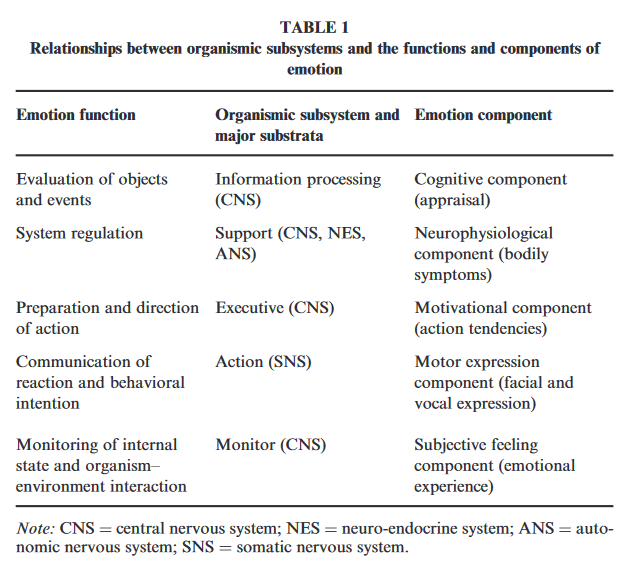
\includegraphics[width=16cm]{Bilder/Relationships-between-organismic-subsystems.png}
	\label{img:Emotion}
	\caption[Relationships between organismic subsystems and the functions and components of
	emotion - Klaus R. Scherer]{Relationships between organismic subsystems and the functions and components of
		emotion - Klaus R. Scherer\footnotemark}
\end{figure}%
\footcitetext[Vgl.][S.698 Table 1]{Kla05}
Anhand dieser Tabelle lässt sich eine Unterscheidung zwischen dem Begriff Gefühl und Emotion durchführen. Der Unterschied ist das ein Gefühl eine einzelne Komponente der Emotion ist, welche erst in Verbindung mit anderen Emotionskomponenten zu einer Emotion führt. 
\subsubsection{Wie lassen sich Emotionen messen?}
\subsubsectionauthor{Torben Brenner}
Nach dem nun geklärt ist wie eine Emotion aufgebaut ist, müssen wir uns die Frage stellen, wie es möglich ist eine Emotion zu messen. Der naheliegendste Ansatz ist zu versuchen, die einzelnen Emotionskomponenten messbar zu machen. Das dies nicht so einfach umzusetzen ist, zeigt die Betrachtung der kognitiven Emotionskomponente. Diese steht im direkten Zusammenhang mit dem zentralen Nervensystem (siehe \ref{img:Emotion} S.\pageref{img:Emotion}). Eine Messung der Veränderungen in diesem System ist äußerst kompliziert und insbesondere in unserem Anwendungsfall nicht möglich. Daher muss ein anderer Ansatz untersucht werden Emotionen zu messen.
\subsubsection{Geneva Emotion Wheel}
\subsubsectionauthor{Torben Brenner}
Das \textit{Geneva Emotion Wheel} baut auf dem Ansatz auf, die Emotionen anhand verschiedener Dimensionen zu bestimmen. In einem Prototyp für das \textit{Geneva Emotion Wheel} (zu sehen in \ref{img:Geneva} S.\pageref{img:Geneva}) werden die beiden Dimensionen \textit{arousal} und \textit{valence} betrachtet.
\begin{figure}[h]
	\centering
	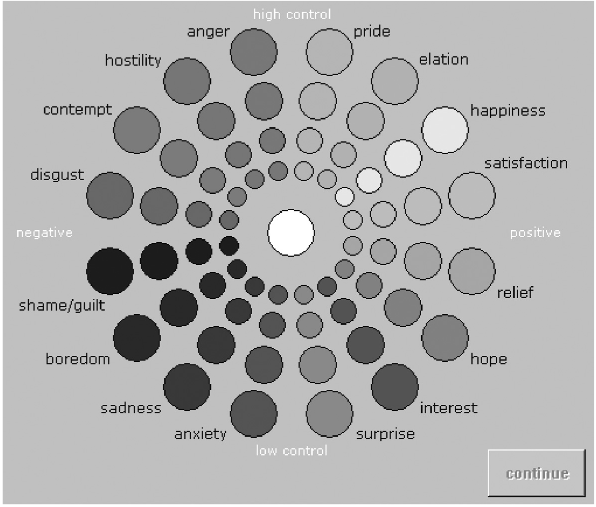
\includegraphics[width=16cm]{Bilder/Geneva-Emotion-Wheel.png}
	\label{img:Geneva}
	\caption[Prototype version of the Geneva Emotion Wheel - Klaus R. Scherer]{Prototype version of the Geneva Emotion Wheel - Klaus R. Scherer\footnotemark}
\end{figure}%
\footcitetext[Vgl.][S.723 Figure 2]{Kla05}
Die erste Dimension bezeichnet wie stark die Erregung eines Individuums ausgeprägt ist in einer Situation. Die zweite Dimension gibt an wie Unwohl sich ein Individuum in einer Situation fühlt. Beide Dimensionen haben gemeinsam, dass sie durch die Befragung eines Individuums ermittelt werden müssen.
\subsubsection{Rad der Emotionen nach Robert Plutnick}
\subsubsectionauthor{Torben Brenner}
Nach dem nun geklärt ist was unter einer Emotion verstanden wird, stellt sich die Frage wie man diese erkennen kann. Das Problem hierbei ist, dass es eine große Anzahl an Emotionen gibt, laut Hokuma\footcite[Vgl.][Absch. 1]{Hok17} sind es 34.000 unterschiedliche Emotionen. Diese verschiedenen Emotionen lassen sich nur schwer erfassen und unterscheiden, weshalb ein Weg gefunden werden muss die Emotionen einzuteilen. Diese Einteilung wurde bereits von Robert Plutchick vorgenommen und herausgekommen sind dabei acht primäre Emotionen: Freude, Traurigkeit, Akzeptanz, Ekel, Angst, Wut, Überraschung und Erwartung.\newline
Mit diesen acht Emotionen hat Plutchick das Rad der Emotionen gebildet(siehe Abbildung).
\begin{figure}[h]
	\centering
	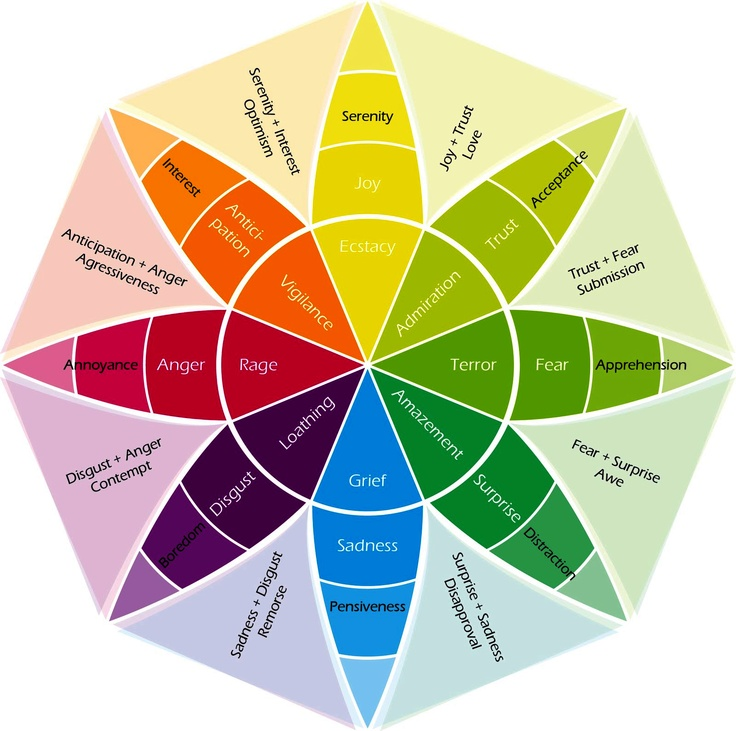
\includegraphics[width=16cm]{Bilder/wheel-of-emotions.png}
	\caption[Rad der Emotionen - Robert Plutchick]{Rad der Emotionen - Robert Plutchick\footnotemark}
\end{figure}%
\footcitetext[Vgl.][]{Hok17}
\newline
Das Rad stellt die primären Emotionen dabei in Relation, wobei die Kombinationen zwischen zwei Emotionen im Raum zwischen diesen steht und Emotionen die gegensätzlich wirken, z. Bsp. Traurigkeit und Freude, jeweils auch gegenüberliegend auf dem Rad sind. Außerdem wird die Stärke einer Emotion durch deren nähe zum Zentrum des Rads gekennzeichnet, z. Bsp. Wut zu toben \footcite[Vgl.][Absch. Elements of the Wheel]{Hok17}.\newline
\subsection{Umgang mit biometrischen Daten}
\subsectionauthor{Torben Brenner}
Eine Problematik, mit der wir uns in dieser Arbeit beschäftigen müssen, ist der Umstand das biometrische Daten nicht immer einen direkten Schluss auf einen Emotion zulassen. So lässt ein hochfrequenter Puls keinen direkten Schluss auf die Emotion zu, die ein Individuum gerade empfindet. Er kann maximal ein Indiz für verschiedene Emotionen sein, z. Bsp. Wut oder Angst. Um mit diesem Umstand umzugehen benötigen wir zwei neue Begriffe die im folgenden genauer erläutert werden. 
\subsubsection{Indiz}
Ein Indiz ist im allgemeinen Sprachgebrauch ein Anzeichen für einen Umstand, an dem sich ein Zustand oder eine Entwicklung absehen lässt\footcite[Vgl.][]{Dud18}. In unserer Arbeit, sehen wir Daten die wir von den Sensoren bekommen, als Indizien an. Ein Indiz macht es wahrscheinlicher bzw. unwahrscheinlicher das ein Individuum eine bestimmte Emotion verspürt. 
\subsubsection{Kausalität}
Als Kausalität wird im allgemeinen der Zusammenhang zwischen Ursache und Wirkung verstanden. In der Physik ist die Kausalität ein grundlegendes Prinzip, welches besagt, ``daß in der Natur nichts ohne Grund passiert, d.h. zu jedem Ereignis (Wirkung) ein anderes (Ursache) existiert, das a) in seiner Vergangenheit liegt und b) zwingende Voraussetzung für das Eintreten der Wirkung ist''\footcite{Sav18}.\newline
In dieser Arbeit werden wir ebenfalls versuchen, kausale Zusammenhänge zwischen Reaktionen des Körpers und den gerade empfundenen Emotionen zu ermitteln.
Ein Werkzeug um kausale Zusammenhänge darzustellen ist in der Literatur der Kausale Graph (im englischen \textit{directed acyclic graph}).
\begin{figure}[h]
	\centering
	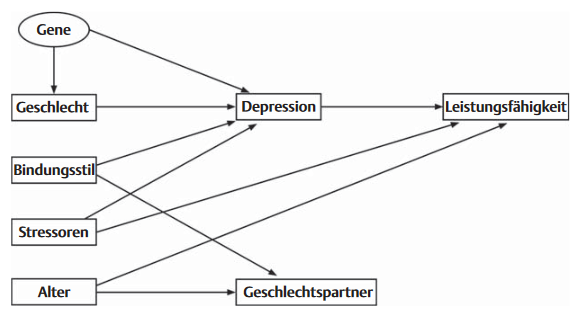
\includegraphics[width=11cm]{Bilder/dag.png}
	\caption[Fiktives Beispiel eines DAGs]{Fiktives Beispiel eines DAGs\footnotemark}
\end{figure}
\footcite[Vgl.][Kausale Graphen - DAGs]{Tho11}
Die Grafik zeigt ein fiktives Beispiel für einen kausalen Graphen. In diesem Beispiel von Thoemmes wird dargestellt das Bindungsstil, Geschlecht, Stressoren und Gene Einfluss auf Depressionen haben. Wichtig ist, dass alle Annahmen die in einem solchen Graph gemacht werden theoretisch begründet werden müssen. Ist dies nicht der Fall, dürfen sie kritisiert und infrage gestellt werden \footcite[Vgl. ][S.3 Kausale Graphen - DAGs]{Tho11}.
\subsection{Emotionsindizien}
\subsectionauthor{Torben Brenner}
\label{section:Emotionsindizien}
Dieser Abschnitt beschäftigt sich mit der Frage, welche biometrischen Merkmale existieren und inwiefern sie sich zur Bestimmung von Emotionen eignen. Daten die sich zur Bestimmung von Emotionen eignen nennen wir Emotionsindizien, da sie einen Hinweis auf die empfundenen Emotionen einer Person liefern.
\subsubsection{Puls}
\subsubsectionauthor{Torben Brenner}
% Was verstehen wir unter dem Begriff Puls
In diesem Abschnitt beschäftigen wir uns mit dem Puls als ein Indiz für verschiedene Emotionen. Hierbei wird der als der biologische Puls gesehen, das heißt ``die in Abhängigkeit vom Herzrhythmus (Herzmechanik) erfolgende Schwankung von Blutstrom, Blutdruck oder Blutvolumen im Blutkreislaufsystem (Blutgefäßsystem, Blutkreislauf)''\footcite{Spe18}. Neben dieser Definition wird im Lexikon der Biologie auch folgende Definition genannt: ``die vom Herzschlag bewirkte, rhythmisch auftretende Druckwelle (Pulsschlag) in den Arterien''\footcite{Spe18}, welche den Puls als arteriellen Puls definiert. \newline
% Wie wird der Puls gemesen? Ruhepuls nicht Ruhepuls(Sphygmologie)
Es gibt mehrere Möglichkeiten den Puls zu messen. Die häufigste Methode, welche auch in Erste-Hilfe-Kursen gelehrt wird, ist die Messung des Pulses an der Arterie. Das Grundprinzip ist dabei, dass die vom Herzschlag verursachte Druckwelle an der Arterie für Menschen spürbar ist und somit dort mitgezählt werden kann.\newline
% Wie lässt sich der Puls als Biometrisches Merkmal einordnen?
Der Puls ist in der Biometrie als ein physiologisches Merkmal zu sehen. Eine Person muss keine speziellen Handlungen durchführen um einen Puls zu haben. Der Aspekt der \textit{Universalität} ist bei diesem Merkmal gegeben, da jeder Mensch einen Puls besitzt. Eine Erfassung des Pulses ist quasi jeder Zeit möglich, zumindest für Menschen. Ein Smartphone bietet aber auch mehrere Möglichkeiten den Puls zu messen, die später in dem Abschnitt ``Erfassung der biometrischen Daten'' weiter erläutert werden. Der Aspekt der Permanenz ist nicht vollständig gegeben. Der Puls bewegt sich zwar standardmäßig in einem bestimmten Wertebereich, ist aber abhängig von Alter und körperlicher Verfassung einer Person.\newline
% In wie fern kann der Puls als Indiz verwendet werden?
Als Emotionsindiz kann der Puls unterstützend wirken, da dieser eine physiologische Auswirkung von verschiedenen Emotionen sein kann. Dennoch ist er kein alleiniges Merkmal für eine bestimmte Emotion, da sowohl Freude als auch Angst einen erhöhten Puls zur folge haben können.
\subsubsection{Hautleitfähigkeit/Hautwiderstand}
\subsubsectionauthor{Lukas Seemann}
Die menschliche Haut verfügt über \glqq \textit{aktive als auch passive elektrische Eigenschaften, die sich auf Strukturen und Fuktionen der Haut und der in ihr enthaltenen Organe zurückführen lässt.}\grqq{}\footcite[][S. 2]{Bou88} Diese elektrischen Phänomene der Haut sind in wissenschaftlichen Kreisen unter dem Sammelbegriff elektrodermale Aktivität (kurz EDA) bekannt. \footcite[Vgl.][S. 2]{Bou88}
Eine elektrodermale Aktivität, die sich sehr gut als Indikator für Emotionen eignet, ist die Hautleitfähigkeit. Hierzu wird mit einer externen Stromquelle mit geringer Spannung gemessen, wie gut die Haut eines Probanden diesen Strom leitet. \footcite[Vgl. ][S.77]{Moe07} Häufig wird anstand der Hautleitfähigkeit auch der Hautwiderstand gemessen. Diese beiden Indizien stehen in einer negativ proportionalen Beziehung. Dies bedeutet, je höher der Widerstand der Haut ist, desto niedriger ist die Leitfähigkeit und umgekehrt. Letzten Endes sagen beide Indizien dasselbe aus, unterscheiden sich aber in der Betrachtungsrichtung. \footcite[Vgl. ][S. 28]{Die06} \newline
Die Hautleitfähigkeit wird anhand der Menge von Schweiß an den Ausgängen der Schweißdrüßen bestimmt, die sich über den gesamten Körper veteilen. Je mehr Schweiß, der elektrisch sehr gut leitend ist, sich auf der Haut befindet, umso größer ist die Hautleitfähigkeit. Am besten eignen sich  Stellen, an denen die Schweißdrüsen sehr dicht angeordnet sind und die somit sehr schweißsensibel sind. Dies ist zum Beispiel an den Handinnenflächen beziehungsweise Fingerinnenseiten der Fall, die sich deshalb sehr gut für solche Messungen eignen. \footcite[Vgl. ][S.77]{Moe07} 
\begin{figure}[h]
	\centering
	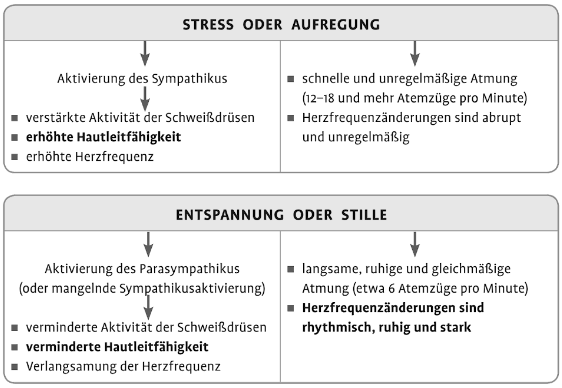
\includegraphics[width=14.6cm]{Bilder/symp.png}
	\caption[Reaktion des Körpers auf Stress und Entspannung]{Reaktion des Körpers auf Stress und Entspannung\footnotemark}
\end{figure}%
\footcitetext[][S. 200]{Dil13}
\newline
\glqq \textit{Die Aktivation beschreibt das Ausmaß der physiologischen Aktiviertheit oder Wachheit eines Menschen}\grqq{}\footcite[][S. 28]{Die06}. Unter Aktivitation versteht man bei Menschen generell jede Art von emotionaler Erregung. Hierzu zählen unter anderem Wut, Aufregung, Schreckmomente oder auch extreme Freude. In Abbildung 3 ist die Reaktion des Körpers auf Stress (darausfolgend auch Aktivation) und auf Entspannung dargestellt. Die Schweißprodukation wird über das unwillkürliche Nervensystem gesteuert. Dieses besteht aus Sympathikus der für die Bereitstellung von Energie und Arbeitsleistungs zustöndig ist, und dem Parasympathikus, der zur Erholung und Wiederherstellung von Körperfunktionen dient. \footcite[Vgl. ][S. 5]{Lie13} \newline Bei Stress oder Aufregung wird der Sympathikus aktiviert, was eine versträkt Schweißproduktion und somit auch eine erhöhte Hautleitfähigkeit hervorruft. Außerdem wird die Herz- und Atemfrequenz erhöht und der Rhymtmus dieser ist unregelmäßig. Die Reaktion auf ein Ereignis, das emotionale Erregung hervorruft, lässt sich meistens innerhalb von einer bis vier Sekunden anhand der Änderung der Hautleitfähigkeit feststellen. \footcite[Vgl.][S. 130f]{Sch14} \newline 
Bei Entspannung hingegen wird der Parasympathikus aktiviert, was zu einer verminderten Aktivität der Schweißdrüßen führt. Die Hautleitfähigkeit sinkt somit auch. Des Weiteren werden Herz- und Atem verlangsamt und gelangen wieder in einen normalen Rhymthmus. \newline
Der Vorteil der Messung der Hautleitfähigkeit ist, dass diese unwillkürlich gesteutert wird und somit keine willentliche Mitarbeit des Probanden erfodert. Da die Aktivierung des Sympathikus automatisch geschieht, kann der Proband die Messung nicht verfälschen. \newline
Ein Nachteil des Verfahren ist, dass die Hautleitfähigkeit nur Rückschlüsse auf den Grad der Aktiviation schließen lässt, jedoch nicht gesagt werden kann, ob es sich um positive oder negative Reaktionen handelt. Die Wut über ein Ereignis würde zum selben Ergebnis führen, wie die übermäßige Freude über ein Ereignis. Aus diesem Grund müssen zur genauen Emotionsbestimmung weitere Indizien herangezogen werden. \footcite[Vgl. ][S.77]{Moe07}
\subsubsection{Mimik}
\subsubsectionauthor{Torben Brenner}
% Was bezeichnet der Gesichtsausdruck
Der Begriff Mimik bezeichnet Bewegungen der Gesichtsmuskulatur mit dem Ziel, eine Emotion auszudrücken. Das nicht jede Gesichtsregung automatisch auch als Mimik gewertet werden kann sieht man beispielsweise beim Kauen \footcite[Vgl. ][Mimik: Eine kurze Definition]{Kar18}.\newline
% In wiefern kann sie als biometrisches Merkmal gewertet werden
Der Vorteil der Mimik als Emotionsindiz ist, dass sie als eines der wenigen Indizien für direkte Aussagen zu den Emotionen gewählt werden kann. So ist es dem Menschen zum Beispiel möglich, alleine durch Beobachtung einer anderen Person Vermutungen anzustellen, welche Emotionen diese gerade empfindet\footcite[Vgl. ][Die sieben Grundemotionen, Absatz 1]{Kar18}. Eine Untersuchung die diese Aussage zusätzlich unterstützt ist der FEEL-Test\footcite[][]{Kes02}. FEEL steht für Facial Expressed Emotion Labeling und ist ein Computerprogramm das auf den Arbeiten von Ekman\footcite{Ekm92} aufbaut. Bei dem Test werden den Probanden Bilder gezeigt die jeweils eine von sechs Basisemotionen wiederspiegeln. Der Proband soll daraufhin versuchen die Emotionen zu erkenne wobei im Ergebnis die Richtigkeit der Antwort und die Antwortzeit betrachtet werden. Ziel des Tests war es ``objektiv
und reliabel die Fähigkeit eines Probanden erfassen, sechs mimisch kodierte Basisemotionen zu erkennen (Freude, Trauer, Ekel, Angst, Überraschung und Ärger)''\footcite[siehe. ][S.5 Z.11ff]{Kes02}. In einer Pilotstudie mit 77 Teilnehmern konnten die Probanden unterschiedlich gut die verschiedenen Emotionen erkennen: ``(Trauer 
70\%, Angst 71\%, Ekel 80\%, Überraschung 84\%, Freude 87\% und Ärger 94\%)''\footcite[siehe. ][S.9 Z.9f]{Kes02}.\newline
Die Ergebnisse der Studie zeigen, dass Menschen aus der Mimik einen Schluss auf eine Emotion ziehen können. Im Verlauf der Arbeit werden wir untersuchen, ob es Möglichkeiten gibt, mit der Smartphonekamera ebenfalls ein solches Ergebnis erzielen können oder dieses sogar übertreffen können. 
\subsubsection{Tippverhalten}
\subsubsectionauthor{Torben Brenner}
Unter dem Tippverhalten wird die individuelle Art einer Person verstanden, wie sie auf virtuellen oder realen Tastaturen tippt. Dabei wird unter anderem der Eingaberythmus als Erkennungsmerkmal betrachtet\footcite[Vgl. ][Allgemein Abs. 1]{Bio18b}. Die Erkennungsgenauigkeit, und damit auch die Sicherheit des Verfahrens, ist dabei von der Frequenz der abgefragten Werte und der eingestellten minimalsten Ähnlichkeit abhängig. Bei diesem biometrischen Merkmal handelt es sich um ein verhaltensorientiertes Merkmal. Erfassbar ist dieses Merkmal immer, wenn der Nutzer einen vorgegebenen Text eingeben muss und für diesen ein Vergleichsprofil vorhanden ist. Dies kann zum Beispiel auch zur zusätzlichen Prüfung bei der Passworteingabe verwendet werden.\newline
Es gibt wenige Arbeiten die sich mit der Verbindung von Emotionen und dem Tippverhalten beschäftigen. Eine dieser wenigen Arbeiten ist von Trojahn, Arndt, Weinmann und Ortmeier. Diese stellten bezüglich dieses Themas fünf Thesen auf und prüften diese innerhalb ihrer Arbeit\footcite[Vgl. ][S.32 2.3 Hypotheses]{Tro13}. Drei dieser Hypothesen beziehen sich dabei direkt auf die Verbindung zwischen Tippverhalten und Emotionen, weshalb sie hier genannt werden\footcite[siehe ][S.33 Z.8-13]{Tro13}:
\begin{itemize}
	\item \textbf{H3:} [Je langsamer die Tippgeschwindigkeit, desto negativer werden Emotionen wargenommen]
	\item \textbf{H4:} [Je höher die Tippfehlerrate, desto negativer werden Emotionen wargenommen]
	\item \textbf{H5:} [Je höher der Fingerdruck, desto negativer werden Emotionen wargenommen]
\end{itemize}
Um die Hypothesen zu prüfen, führten sie eine Studie mit zwei Samsung Galaxy Nexus Smartphones aus, bei der es die Aufgabe der Probanden war mit Hilfe des Smartphones einen Text einzutippen. Dabei wurden denn Probanden unterschiedliche Zeitgrenzen gegeben um unterschiedliche Ebenen von Stress zu repräsentieren. Nachdem der Test durchgeführt war, sollten die Probanden noch einen Fragetext zu ihren empfundenen Emotionen beantworten\footcite[Vgl. ][S.33 3.1 Study Object and Study Task]{Tro13}. Durch ihre Studie konnten sie zeigen, dass Emotionen durch Tastendrücke beschrieben werden können. In diesem Zusammenhang wurden die Hypothesen 3 und 4 bestätigt, aber Hypothese 5 widerlegt\footcite[Vgl. ][S.35 5.1 Summary]{Tro13}.\newline
Durch diese Studie wurde gezeigt, dass das Tippverhalten ebenfalls als Emotionsindiz gewertet werden, weshalb es auch weiter untersucht werden soll.
\subsubsection{Gangart}
% Was ist die Gangart
Wie bereits im Abschnitt Biometrie und biometrische Merkmale(siehe S.\pageref{section:Biometrie}) erläutert, ist auch die Gangart eines Menschen ein biometrisches Merkmal. Die Gangerkennung setzt dabei darauf, ``dass jeder Mensch eine relativ spezifische Gangart besitzt, an der er unter Zuhilfenahme anthroprometrischer Maße wie Beinlänge und Bein Form nahezu eindeutig erkannt werden kann''\footcite[siehe ][Abschnitt Allgemein Abs.2 Z.2]{Bio18}. So entstehen beim gehen verschiedene sich wiederholende Muster, die sich mit Hilfe von Sensoren erkennen lassen. So existieren mehrere Merkmale, die sich dazu eignen den menschlichen Gang zuerkennen, hier sei z. Bsp. die Schrittweite oder die Schrittzeit genannt.\newline
Verschiedene wissenschaftliche Quellen treffen die Aussage, dass sich Emotionen auch auf die Bewegung einer Person auswirken können. So stellen Walk \& Homan in ihrer Arbeit folgende Theorie auf.
\begin{quote}
	``Although emotion may be expressed in the face, it can also be expressed in the voice and in body movement. People jump with joy or cringe with fear.''\footcite[siehe ][S.437 Z.20-23]{Wal84}
\end{quote}
In ihrer Arbeit haben sie ein Experiment mit 24 Studenten durchgeführt, denen sie Videosequenzen vorgespielt haben in denen zwei verschiedene Schauspielerinnen, verschiedene Körperliche und Emotionale Zustände dargestellt haben. Die Studenten hatten in der ersten Phase des Experiments, die Aufgabe, die gesehenen Videosequenzen zu beschreiben. In der zweiten Phase, in der den Studenten die Aufnahme erneut gezeigt wurde, hatten diese die Aufgabe einzuschätzen wie viele verschiedene Personen sie in dem Video gesehen haben und welches Geschlecht diese haben\footcite[Vgl. ][S.437+438 Method]{Wal84}. Als ein Ergebnis dieses Experiments stellten die Authoren in einer Tabelle(siehe Abbildung) ihre Ergebnisse mit denen von Ekman\footcite{Ekm92} in Vergleich. 
\begin{figure}[h]
	\centering
	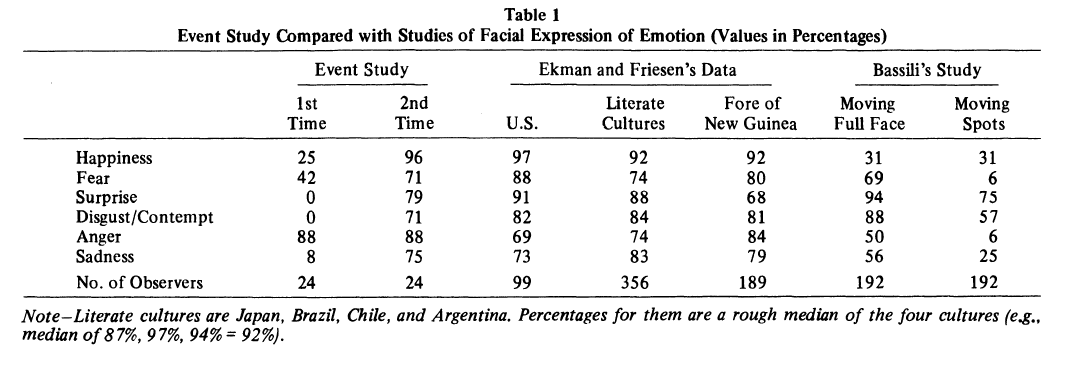
\includegraphics[width=16cm]{Bilder/Gangerkennung-Emotion-Vgl.png}
	\caption[Event Study Compared with Studies of Facial Expression of Motion(Values in Percentages)]{Event Study Compared with Studies of Facial Expression of Motion(Values in Percentages)\footnotemark}
\end{figure}\footcitetext[siehe. ][Tabelle 1 S.438]{Wal84}
In der Grafik ist deutlich zu sehen, dass die Teilnehmer der Studie von Walk \& Homan beim ersten sehen der Videos Probleme hatten, die Emotionen zu erkennen. Einzig die Emotion \textit{Wut} wurde von einem Großteil der Teilnehmer erkannt. Beim zweiten Ansehen des Videos, konnten die Probanden aber deutlich besser die verschiedenen Emotionen erkennen. In diesem Fall war es für die sechs untersuchten Emotionen immer mindestens 70\% möglich die dargestellte Emotion zu erkennen. Im Vergleich mit der Studie von Ekman sind diese Ergebnisse schon deutlich Konkurrenzfähiger. Dennoch scheinen die Probanden anhand der Untersuchungsergebnisse, eher anhand des Gesichtsausdrucks, als den Bewegungen eines Menschen dessen Emotionen erkennen zu können. Dennoch ist hier anzumerken, dass sich die Teilnehmer Anzahl der beiden Studien deutlich unterscheidet und bei dem Experiment von Ekman eine gemischte Personen Gruppe genutzt wurde, während dem Walk \& Homan ausschließlich Studenten und Studentinnen untersuchten.\newline
Dennoch zeigt das oben vorgestellte Experiment das eine Emotionserkennung anhand des Gangs möglich ist und deshalb wird diese Als Emotionsindiz aufgenommen.
\subsubsection{Stimme}
\subsubsectionauthor{Torben Brenner}
% Was ist die Stimme?
% Stimme als biometrisches Merkmal
Die menschliche Stimme kann ebenfalls als biometrisches Merkmal gesehen werden. Dabei ist insbesondere zu beachten, dass bei der Stimme der Faktor \textit{Permanenz} nicht gegeben ist, da diese sich im Verlaufe des Lebens ändert. Dies geschieht über Veränderungen in der Physiologie eines Menschen, z. Bsp. die Stimmbandlänge und die Kehlkopfgröße. Solche Änderungen geschehen unter anderem während dem Alterungsprozess, die stärkste davon in der Pubertät. Das Problem kann aber durch eine ständige Nachkalibrierung während jedem Identifikationsprozesses\footcite[Vgl. ][S.198 Z.22-26]{Til11} behoben werden.\newline
\cite{Pat18} haben in ihrer Arbeit nach möglichen akustischen Merkmalen für Emotionen gesucht. Dazu haben Sie die Aussprache des Vokals ``a'' von zehn unterschiedlichen französischen Schauspielern untersucht. Die Schauspieler haben für die GEMEP Datenbank diesen Vokal jeweils in 12 unterschiedlichen emotionalen Kontexten wieder gegeben\footcite[Vgl. ][S.2 Z.13-16]{Pat18}. Dabei herausgekommen ist, dass einige dieser Merkmale sich dazu eignen, Erregung in der Stimme festzustellen\footcite[Vgl. ][S.4 Z.28-32]{Pat18}. Mit der Erregung lässt sich bereits zwischen einigen Emotionen unterscheiden, weshalb diese auch im \textit{Geneva Emotion Wheel} als eigene Dimension gewählt wurde. Aus diesem Grund ist auch die Analyse der Stimme ein für die Emotionserkennung relevanter Bereich.
\subsection{Nützliche Hardware}
\subsubsection{Smartphones}
\subsubsectionauthor{Torben Brenner}
% Definition Smartphone
Auch wenn der Begriff des Smartphones heutzutage häufig Synonym zu dem des Mobiltelefons verwendet wird, beschreiben die beiden Begriffe dennoch unterschiedliche Gerätearten. Smartphones sind im allgemeinen eine Weiterentwicklung des herkömmlichen Mobiltelefons. Neben der Standardfunktion des mobilen Telefonierens und der Unterstützung des \textit{Short Message Service} (kurz SMS), bieten Smartphones mittlerweile viele weitere Funktionen wie z. Bsp. GPS oder Internetzugriff\footcite[Vgl. ][S.3 Z.5ff]{Bou11}.\newline
% Unterschied zum herkömmlichen Breitband Telefon/Mobiltelefonen
Dieser erhöhte Umfang an Funktionen ermöglicht es, Entwicklern Anwendungen für viele verschiedenen Anwendungsfälle bereitzustellen und somit den Nutzer deutlich besser in seinem Alltag zu unterstützen als mit einem Mobiltelefon\footcite[Vgl. ][Smartphones are tiny Computers]{Ada18}. Eine weitere Entwicklung, die vom Mobiltelefon zum Smartphone stattfand, war die Weiterentwicklung des Betriebssystems. Während Mobiltelefone meist mit simplen Betriebssystemen ausgestattet sind, werden Smartphones von komplexen Systemen wie Android oder IOS angetrieben. Diese bieten Nutzern die Möglichkeit zusätzliche Programme zu installieren wie z.Bsp. bei Windows\footcite[Vgl. ][Mobile Operating Systems]{Ada18}.\newline
% Vergleich Leistung mit einem Computer
Der erhöhte Funktionsumfang von Smartphones im Vergleich zu Mobiltelefonen führt uns zur Frage, ob Smartphones auch dazu genutzt werden können, einen Computer zu ersetzen. Verschiedene Hersteller wie z. Bsp. Samsung mit den Dex-Stationen bieten Nutzern bereits die Möglichkeit, ihr Smartphone als PC-Ersatz zu nutzen\footcite{Kai18}. Obwohl Smartphones immer höhere Leistungsspitzen erreichen, werden sie wahrscheinlich auch in Zukunft nicht als vollständiger PC-Ersatz genutzt werden können. Das liegt insbesondere daran das Smartphone CPUs (Central Processing Unit) aufgrund des Formfaktors nicht so gekühlt werden können wie PC-CPUs\footcite[Vgl. ][Power and Heat]{Gav18}.\newline 
% Warum Smartphones zur Emotionserkennung? Ermöglichen Tagesanalyse/Verbreitung
Nun kommen wir zu der Frage warum wir Smartphones verwenden wollen um Emotionen zu erkennen. Zum einen sind Smartphones in der Lage, durch verschiedenen verbaute Sensoren zu sehen, fühlen und zu hören\footcite[Vgl.][S. 1 Abs. 2]{Bie14}. Wie in dem Artikel beschrieben, geben uns die verbauten Sensoren enorme Möglichkeiten mit dem Smartphone die Umwelt wahrzunehmen. Wie leistungsfähig die verschiedenen Komponenten mittlerweile geworden sind, zeigt Apple mit dem IPhone X, welches mithilfe der Kamera und Infarotsensoren, die Veränderungen von Gesichtszügen erkennt und auf sogenannte Animojis überträgt\footcite[Vgl. ][Animoji: So funktioniert es]{Com17}. Ein weiterer Grund aus dem wir die Emotionserkennung mit Smartphones untersuchen wollen ist die Tatsache, dass Smartphonenutzer ihr Gerät häufig rund um die Uhr bei sich tragen. Dies ermöglicht es für verschiedene Anwendungsszenarien eine Überwachung der Emotionen des Nutzers über den Tag hinweg durchzuführen.
\subsubsection{Smartphone Sensoren}
\subsubsectionauthor{Torben Brenner}
Wie bereits erwähnt, werden in Smartphones mittlerweile massenweise Sensoren verbaut, die eine Umgebungswahrnehmung möglich machen. Eine Auflistung dieser Sensoren stellt Biermann in seinem Artikel für die Zeit Online vor\footcite[siehe ][]{Bie14}.\newline
So nennt er den Beschleunigungssensor, das sogenannte Akzelerometer. Bei diesem wird mithilfe eines kleinen Siliziumstabs und einer Elektrode die Beschleunigung gemessen. Diese Konstruktion wird dreimal verwendet um für die x-,y- und z-Achse eine Beschleunigungsbestimmung durchführen zu können.\newline
Das Gyroskop ist ein weiterer Sensor, der in Smartphones platz findet. Dieser dient dazu, mit Hilfe von in Schwingung versetzten Metallelementen und Kondensatoren, zu prüfen, ob das Handy hoch oder quer gehalten wird.\newline
Das sogenannte Magnetometer misst auf der X-, Y- und Z-Achse die Stärke und Richtung des Erdmagnetfeldes. Laut Biermann ist z. Bsp. im iPhone 4 ein solcher Sensor verbaut. Dieser kann unter anderem dazu genutzt werden, Stromleitungen in einer Wand zu finden.\newline
Der Touchscreen selbst ist ebenfalls ein Sensor. Dieser besteht aus zwei Gittern, zwischen denen ständig Stromsignale ausgetauscht werden. Dabei wird von der oberen Schicht ein Impuls an die untere Schicht gesendet. Durch Berührung mit dem Finger, und dessen Feuchtigkeit, wird das Signal lokal schwächer. Diese Veränderung wird von einem Prozessor zur Position des Fingers umgerechnet.\newline
Dies war nur eine kleine Auswahl aller Sensoren die in Smartphones verbaut sind. Neben den genannten Sensoren werden z.Bsp. auch die Kamera und das Mikrofon als Sensoren verstanden. Diese werden aber in späteren Kapiteln noch einmal genauer beschrieben.
\subsubsection{Externe Sensoren}
\subsubsectionauthor{Torben Brenner \& Lukas Seemann}
Da es nicht möglich ist, alle Indizien die in Kapitel 2.4 aufgezählt wurden mithilfe der Smartphone-internen Sensoren zu erfassen, müssen zusätzliche externe Sensoren zur Erfassung von biometrischen Daten hizugezogen werden. \newline
Sensoren dienen zur Erfassung eines physikalischen Zustandes und der Transformation dieses Zustandes in einen Impuls, der verarbeitet werden kann\footcite[Vgl.][]{Web18}. In der Computertechnik dienen Sensoren häufig dazu, den physikalischen Zustand verständlich für einen Computer zu machen, indem dieser in einen Datensatz umgewandelt wird. Generell sind für einen Computer elektrische Signale erkennbar, jedoch sind nicht alle Messgrößen, die am Eingang eines Sensors anliegen elektrisch. Die Aufgabe von Sensoren ist es also, nichtelektrische Messgrößen in ein elektrisches Signal umzuwandeln. \newline
In Abbildung ? ist die Umsetzung dieses Vorgangs gezeigt.
\begin{figure}[h]
	\centering
	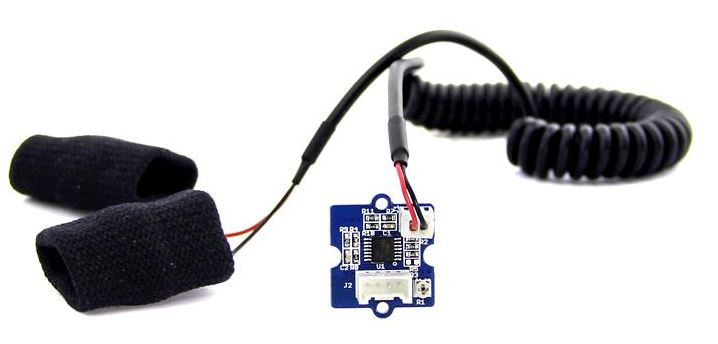
\includegraphics[width=16cm]{Bilder/sensor.png}
	\caption[Sensor als Schnittstelle zwischen nicht-elektrischen und elektrischen Raum]{Sensor als Schnittstelle zwischen nichtelektrischen und elektrischen Raum\footnotemark}
\end{figure}\footcitetext[][S. 347]{Ros13} \newline
Ein Sensor erhält eine nichtelektrische Messgröße als Input und erfasst diese Messgröße mithilfe eines vorgelagerten Primärwandlers. Eine Primärwandler kann je nach Messgröße unterschiedlich gestaltet sein. Bei mechanischen Größen kann es zum Beispiel eine Membran oder ein Biegebalken sein, bei optischen Größen optisch abbildende Systeme wie zum Beispiel eine Linse oder eine Blende. \footcite[Vgl. ][S. 347]{Ros13} \newline Das sogenannte Sensorelement stellt den eigentlichen Sensor dar, der den Übergang von nichtelektrischen in den elektrischen Raum realisiert. Hier geschieht die Umwandlung der Messgröße in ein elektrisches Signal.\footcite[Vgl. ][S. 347]{Ros13} \newline Da die Änderungen der elektrischen Größe am Ausgang des Sensorelements in der Regel sehr klein sind, muss das Signal mittels einer Primärelektronik in ein gut verarbeitbares elektrisches Signal verstärkt werden. Dazu ist häufig eine Hilfsenergie notwendig, die dem Sensor zugeführt werden muss. \footcite[Vgl. ][S. 347]{Ros13} Ist dies geschehen, kann das elektrische Signal des Sensors von Computern analysiert werden.\newline
Eine Möglichkeit, externe Sensoren mit dem Smartphone zu verbinden, ist der Einsatz von Mikrocontrollern, wie zum Beispiel ein Arduino. \footcite[Arduino UNO R3 Mikrocontroller: ][]{Ard18} Da nur wenige externe Sensoren direkt an das Smartphone angeschlossen werden können und Mikrocontroller meist sehr handlich sind, ist diese Möglichkeit sehr praktisch. Der Mikrocontroller übernimmt dann zum einen die Erfassung des elektrischen Signals des Sensors und die Übertragung der Daten zum Smartphone. 
\subsection{Möglichkeiten der Erfassung von biometrischen Daten} 
\subsectionauthorlong{Torben Brenner}
In diesem Abschnitt werden unterschiedliche Möglichkeiten vorgestellt, die in \ref{section:Emotionsindizien} vorgestellten Emotionsindizien zu erfassen. Da es nicht immer nur eine Möglichkeit gibt, diese zu erfassen, werden hier verschiedene Methoden diskutiert. Pro Emotionsindiz wird dann eine Methode ausgewählt, die untersucht werden soll.  
\subsubsection{GSR-/EDA-Sensoren}
\subsubsectionauthor{Lukas Seemann}
Die bereits in Kapitel 2.4.2 beschriebene elektrodermale Aktivität kann mithilfe von EDA-Sensoren gemessen werden. Diese Art von Sensoren sind üblicherweise nicht in Smartphones eingebaut, weswegen die Hautleitfähigkeit mit externer Hardware gemessen werden muss. \newline
Die für heute eher unübliche Messungsart der elektrodermalen Aktivität stellt die endosomatische Messung dar. Indem winzige Elektroden in die Haut eingestochen werden, kann die Aktivität der Nerven in der Haut gemessen werden. \footcite[Vgl.][Folie 25]{Sch12} Hierbei handelt es sich jedoch nicht um eine Messung der Hautleitfähigkeit sondern um eine Messung des Hautpotenzials. \newline
\begin{figure}[h]
	\centering
	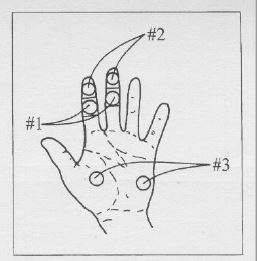
\includegraphics[width=10cm]{Bilder/gsr-hand.jpg}
	\caption[Positionsmöglichkeiten der EDA-Messung]{Positionsmöglichkeiten der EDA-Messung\footnotemark}
\end{figure}\footcitetext[][Folie 25]{Sch12}
\newline
Bei der exosomatischen Messung hingegen wird ein schwacher Strom von ungefähr 0.5 Volt an die Haut angelegt. Die Spannung wird hierbei konstant gehalten, wodurch die Leitfähigkeit der Haut gemessen werden kann. Hierbei gemessen wird entweder in der Einheit Siemens für den elektrischen Leitwert oder in Ohm für den Widerstand. Die Elektroden des Sensor sind meistens aus Silber oder Silberchlorid und werden meist an zwei Stellen der nicht dominanten Hand angebracht. \footcite[Vgl.][Folie 25]{Sch12} Wie in Abbildung ? dargestellt gibt es verschiedenen Möglichkeiten der Handinnenfläche, die gut geeignet sind, (\#1, \#2 oder \#3). \newline
Diese Art von Sensoren sind die heutzutage übliche Vorgehensweise bei EDA-Messungen. Häufig sind sie auch unter dem Namen GSR-Sensor\footnote{GSR: Galvanic Skin Response} bekannt und darunter im Internet erhältlich. GSR-Sensoren sind als Modul für den Mikrocontroller Arduino verfügbar.\footcite[beispielsweise:][]{Gro18} Dies stellt eine Möglichkeit dar, einem mobilen Endgerät die Sensordaten zum Beispiel über Bluetooth oder WiFi zur Verfügung zu stellen. In Abbildung ? ist ein GSR-Sensor inklusive der Elektroden für die Fingerinnenseiten, der mit Arduinos kompatibel ist, abgebildet.
\begin{figure}[h]
	\centering
	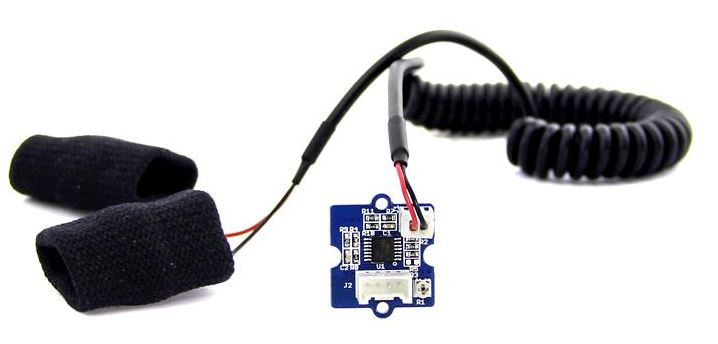
\includegraphics[width=15cm]{Bilder/sensor.jpg}
	\caption[GSR-Sensor mit Finger-Elektroden]{GSR-Sensor mit Finger-Elektroden\footnotemark}
\end{figure}%
\footcitetext{Gro18}
\subsubsection{Stimmerkennung mit Smartphone-Mikrofon}
Grundsätzlich haben alle Smartphones ein Mikrofon, da dieses insbesondere für das Telefonieren gebraucht wird. Biermann schreibt in seinem Artikel außerdem davon, dass heutige Smartphones nicht nur ein Mikrofon, sondern gleich mehrere Mikrofone besitzen. Die zusätzlichen Mikrofone werden unter anderem dazu verwendet, Störgeräusche herauszufiltern\footcite[Vgl. ][S.2 Mikrofon Abs.2]{Bie14}.\newline
Das die Stimmerkennung sich im allgemeinen immer weiterentwickelt, zeigen so genannte \textit{Vocal Computing} Schnittstellen. Dieser Begriff bezeichnet laut Ferdinand und Jetzke ``die Möglichkeit, über Sprache mit Computern, mobilen und stationären Endgeräten sowie deren softwarebasierten Anwendungen zu interargieren''\footcite[siehe ][S.1 Z.1ff]{Fer17}. War es früher noch schwer möglich einzelne Wörter zu erkennen, gibt es mittlerweile Smartphone Anwendungen wie Apples ``Siri'' und Googles ``Google Now'', ``die nicht auf einzelne Befehle reduziert [sind], sondern ganze Sätze und den Kontext ihrer Äußerung erfassen [können]''\footcite[siehe ][S.1 Z.17ff]{Fer17}.\newline
Das auch in der Emotionserkennung über die Stimme ein Fortschritt erreicht wurde, zeigen Russische Forscher mit einem KI-Algorithmus\footcite[Vgl. ][]{Sta17}. Der Algorithmus versucht im Allgemeinen zwischen acht verschiedenen Basisemotionen zu unterscheiden. Dabei scheint es insbesondere bei der Unterscheidung zwischen Freude und Ärger Probleme zu haben. Diese zeichnen sich beide durch eine starke Erregung aus. Wie bereits bei der Beschreibung der Stimme als Emotionsindiz erwähnt, ist dies eines der Hauptmerkmale die sich über die Stimme erfassen lassen.\newline
Das sich solche Anwendungen auch in Form einer Smartphone App umsetzen lassen, haben Ingeneure der University of Rochester gezeigt\footcite[Vgl. ][]{Wed12}. Diese untersuchen in ihrem Programm zwölf unterschiedliche Charakteristiken in gesprochenen Worten, um so zwischen sechs unterschiedlichen Emotionen unterscheiden zu können. Ein App Prototyp zeigt anscheinend schon je nach Stimme einen traurigen oder fröhlichen Smiley an.
\subsubsection{Gesichtserkennung mit Smartphone-Kamera}
\subsubsectionauthor{Torben Brenner}
Zur Erfassung der Mimik, benötigt das Smartphone die Fähigkeit ein Gesicht zu erfassen und den Gesichtsausdruck zu erfassen. Hierfür eignet sich  die Kamera des Smartphones. Diese war früher ausschlieslich für das machen von Bildern gedacht. Mittlerweile werden aber die in Smartphones verbauten Kameras immer besser und können unter anderem für die Gesichtserkennung oder die Verfolgung der Augenbewegungen genutzt werden\footcite[Vgl. ][Seite 2 Kamera Abs. 1+2]{Bie14}.\newline % Warum eignet sich die Handykamera?
\cite{Can01} beschreibt in seiner Arbeit ein Verfahren, um mit Kameras die menschliche Mimik automatisiert zu analysieren. Basierend auf seinen Methoden, kann ein System entwickelt werden, das aus der Mimik eines Menschen dessen Emotionen analysiert. Canzler beschreibt in seiner Arbeit folgende vier Phasen der Analyse\footcite[Vgl. ][S.2-5]{Can01}:
\begin{itemize}
	\item[1.] \textbf{Gesichtsdetektion}
	\item[2.] \textbf{Tracken charakteristischer Punkte}
	\item[3.] \textbf{Extraktion von Mermalen}%in publikation Mermalen
	\item[4.] \textbf{Gesichtsanalyse}
\end{itemize}
Die vier von Canzler ausgearbeiteten Phasen können bis auf wenige Anpassungen übernommen werden. Die Gesichtsdetektion wird mit Hilfe von verschiedenen Verfahren durchgeführt. Die formorientierten Verfahren suchen nach Kanten und Konturen welche dem menschlichen Gesicht entsprechen und farborientierten Verfahren die nach charakteristischen menschlichen Hautfarben suchen\footcite[Vgl. ][S.2 Z.14ff]{Can01}. In der zweiten Phase wird anhand eines vordefinierten durchschnittlichen Gesichts eine Verfolgung von wichtigen Punkten durchgeführt. % Hier wäre es cool über den susan edge kantendetektor zu 
Basierend auf den geometrischen Eigenschaften des Gesichts können daraufhin mit Template Matching verschiedene Merkmale, wie z. Bsp. die Blickrichtung und Stirnfaltenbildung, extrahiert werden. In der letzten Phase, der Gesichtsanalyse, werden die vorher ermittelten Merkmale in sogenannte \textit{Action Units} umgesetzt\footcite[Vgl. ][S.4 Z.17-21]{Can01}. Diese wurden im \textit{Facial Action Coding System} definiert. Sie beschreiben die kleinsten sichtbaren Einheiten von Muskulatur im Gesicht\footcite[Vgl. ][S.94 Z.9ff]{Kai98}. Die Action Units wurden bereits von verschiedenen Forschern in Zusammenhang mit den Emotionen gebracht. Problematisch ist aber laut \cite{Kai98}, dass vollständig vordefinierte Gesichtsausdrücke selten genauso in der Realität vorkommen, weshalb es sinnvoller ist den Zusammenhang zwischen einzelnen AUs und bestimmten Emotionen zu untersuchen\footcite[Vgl. ][S.94 Z.16-30]{Kai98}. Kaiser \& Scherer haben in ihrer Arbeit z. Bsp. das auftreten verschiedener AUs in Zusammenhang mit emotionalen Störungen wie Depressionen beschrieben\footcite[Vgl. ][S.95 Table 6.3 Facial Action Units Predicted as Indicators of Selected Types of Affect Disorders]{Kai98}.
Es gibt bereits mehrere Systeme, die es ermöglichen mit der Analyse des Gesichts Emotionen zu bestimmen. So gibt es vom Fraunenhofer-Institut für Integrierte Schaltungen das SHORE System\footcite[Vgl. ][]{Fra18}. Dieses ermöglicht die Gesichtsanalyse ohne Internetanbindung. Dabei lassen sich sowohl das Geschlecht und Alter, als auch vier unterschiedliche Emotionen erkennen. Es soll außerdem auch auf mobilen Endgeräten funktionieren. Es gibt eine kostenlose Demo, die aber auf eine Laufzeit von 90 Tagen beschränkt ist, weshalb sie sich für unsere Zwecke nicht eignet\footcite[Vgl. ][]{Fra18b}.\newline
Da Smartphones sich unter anderem durch die Möglichkeit auszeichnen, sich unterwegs mit dem Internet zu verbinden ist auch die Nutzung einer Server Anwendung denkbar. Microsoft bietet z. Bsp. eine Schnittstelle für die Gesichtserkennung\footcite[Vgl. ][]{Mic18}. Diese bietet nicht nur die Möglichkeit, Personen zu erkennen und deren Alter zu bestimmen, sondern ermöglicht es auch die Emotionen einer Person zu schätzen. Die kostenlose Nutzung erlaubt 30.000 Transaktionen im Monat mit bis zu 20 Transaktionen in der Minute\footcite[Vgl. ][]{Mic18b}.
\subsubsection{Pulsmessung mit Smartphone-Kamera}
\subsubsectionauthor{Lukas Seemann}
In den App-Stores werden heutzutage mehrere Apps angeboten, die angeben, eine Pulsmessung ohne zusätzliche Geräte zu ermöglichen. \footcite[Vorstellung von Pulsmessungs-Apps auf dem Markt: Vgl.][]{Pet17} Diese Apps nutzen lediglich die im Smartphone integrierte Kamera. Das Ergebnis wird deutlich genauer, wenn das Smartphone außerdem über ein LED-Blitzlicht verfügt.\footcite[Vgl.][]{Gil14} \newline
Die Vorgehensweise bei dieser Art der Pulsmessung ist nicht komplex. Der Smartphone-Nutzer muss dazu lediglich die oberste Fingerkuppe eines beliebigen Fingers auf die Kamera und falls vorhanden auch auf das Blitzlicht des Smartphones legen. Ist kein Blitzlicht vorhanden, ist es auch möglich, die Messung bei gutem Tageslicht durchzuführen.\footcite[Vgl.][]{Gil14} Dies kann jedoch Auswirkungen auf die Genauigkeit des Ergebnisses haben. Über ein gewissen Zeitraum, der meistens im Sekunden- oder niedrigen Minutenbereich liegt, werden anschließend die Helligkeitsschwankungen in der Fingerkuppe des Nutzer aufgezeichnet.\footcite[Vgl.][]{Pre16} Diese Helligkeitschwankungen werden durch den Puls des Benutzer ausgelöst, da der Finger bei hoher Durchblutung nicht so lichtdurchlässig ist, wie bei niedriger Durchblutung. Aus diesen dokumentierten Schwankungen berechnen die Apps mithilfe von signalanalytischen Methoden den Puls des Benutzers. \footcite[Vgl.][]{Pre16} \newline
Diese Methoden sind bereits teilweise laut App-Hersteller-Angaben medizinisch anerkannt\footcite[Vgl.][]{Pre16} und liefern unter guten Bedingung dieselben Ergebnisse, die auch herkömmliche Blutdruckmessgeräte ermittlen würden.\footcite[Vgl.][]{Hen17}
Dieses Verfahren der Pulsmessung basiert auf der Pulsoxymetrie. Das Ziel der Pulsoxymetrie ist es, mithilfe von Lichtquellen die Sauerstoffsättigung und die Pulswelle des Probanden zu messen. \footcite[Vgl. ][S. 74]{Deu09} Als Messorte eignen sich hierfür die Ohren, Zehen oder die Finger, was bei der Smartphone-Messung ausgenutzt wurde. \newline 
\glqq \textit{Bei der Pulsoxymetrie werden von einer Lichtquelle 2 unterschiedliche Wellenlängen (im infraroten und roten Bereich) ausgesendet, die nach dem Durchleuchten des Gewebes (z.B. am Finger) von einem Sensor aufgefangen werden.}\grqq{ \footcite[][S. 74]{Deu09} Neben der hierbei durchgeführten Messung der Sauerstoffsättigung kann durch die Absorption des Lichts durch die Pulswelle über die insgesamt aufgefangene Lichtmenge eine Aussage über die Pulswelle des Probanden abgeleitet werden. \footcite[Vgl. ][S. 74]{Deu09} Obwohl die meisten Smartphones keine verschiedenen Lichtwellenlängen verwenden, sind bereits die Messungen mit dem Blitzlicht des Smartphones für den Puls sehr aussagekräftig. Die unterschiedlichen Lichtwellenlängen sind vor allem für die Sauerstoffsätigung notwendig, deren Messung die meisten Apps nicht anbieten. \newline \newline
Des Weiteren gibt es noch eine weitere Möglichkeit, wie die Smartphone-Kamera zur Pulsbestimmung genutzt werden kann. Mithilfe der Eulerschen Videoverstärkung (\textit{Eulerian Video Magnification}, kurz EVM), die am Massachusetts Institute of Technology (MIT) von einer Gruppe von Informatikern entwickelt wurde, können kleinste Bewegungen in Videomaterial verdeutlicht werden. \footcite[Vgl. ][]{Dam12} Mit einer Videoaufnahme des Gesichts eines Probanden kann so der Puls mit einer hohen Genauigkeit bestimmt werden. Durch die pulsierende Blutzirkulation ändert sich die Gesichtfarbe einer Person ungefähr einmal pro Sekunde. Dies ist mit bloßem Auge nicht sichtbar, kann jedoch mit Hilfe von EVM verstärkt und somit deutlich sichtbar gemacht werden. Mithilfe dieser Farbtonschwankungen kann der Puls sogar in Echtzeit bestimmt werden. \footcite[Vgl. ][]{Dam12} \newline
\begin{figure}[h]
	\centering
	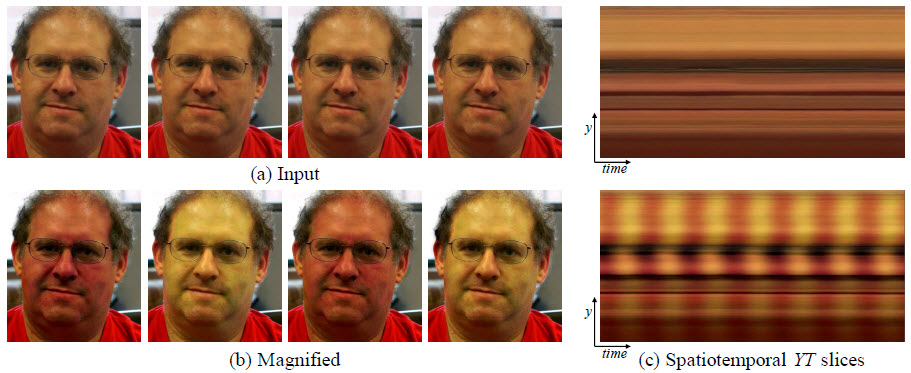
\includegraphics[width=16cm]{Bilder/evm.jpg}
	\caption[Eulersche Videoverstärkung zur Pulsbestimmung]{Positionsmöglichkeiten der EDA-Messung\footnotemark}
\end{figure}\footcitetext{MIT15} \newline
In Abbildung ? ist die Vorgehensweise bei der Pulsbestimmung gezeigt. Zunächst wird das aufgenommene Videomaterial in einzelne Frames unterteilt (siehe \textit{(a)}). Die einzelnen Frames werden dann mithilfe von EVM verstärkt, sodass die durch die Durchblutung veränderte Gesichtfarbe deutlich wird (siehe \textit{(b)}). Rot deutet dabei auf eine hohe Durchblutung hin, wohingegen eine blasse Farbe eine niedrige Durchblutung bedeutet. In \textit{(c)} wird anschließend ein Graph angefertigt, der Ausschnitte des Gesichts im Verlauf der Zeit anzeigt. Bei nicht verstärktem Input sind keine Unterschiede sichtbar. Mit EVM kann jedoch deutlich ausgemacht werden, wie sich die Gesichtsfarbe im Verlauf der Zeit geändert hat. Auf Basis dieses Graphen kann anschließend der Puls bestimmt werden. \footcite[Vgl.][]{MIT15} \newline
Da Smartphones heutzutage über sehr gute Kameras verfügen, kann die Nutzung von EVM eine gute Möglichkeit zur Pulsbestimmung darstellen.
\subsubsection{Pulsmessung mit externen Sensoren}
\subsubsectionauthor{Lukas Seemann}
Neben der Pulsmessung über die Smartphone-Kamera gibt es auch die Möglichkeit, mit externen Sensoren den Puls zu messen. Hierbei gibt es wie auch bei den GSR-Sensor passende Module, die an einen Arduino-Mikrocontroller angeschlossen werden können. \newline
In Abbildung ? ist ein häufig verwendeter Puls-Sensor des Unternehmens World Famous Electronics llc. zu sehen, der mit einem Arduino verbunden werden kann. \newline
\begin{figure}[h]
	\centering
	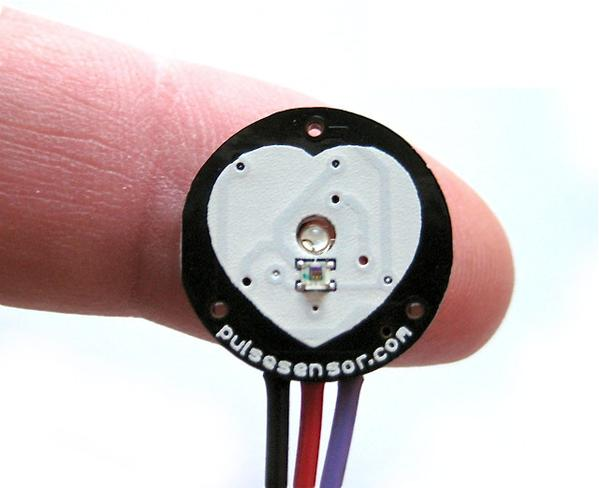
\includegraphics[width=9cm]{Bilder/pulsesensor.jpg}
	\caption[Puls-Sensor für einen Arduino]{Puls-Sensor für einen Arduino\footnotemark}
\end{figure}\footcitetext{Wor18a} \newline
Dieser Sensor kann entweder am Finger oder am Ohr des Probanden angebracht werden. Das Messverfahren basiert hierbei ebenfalls auf der Pulsoxymetrie, es handelt sich also um einen optischen Sensor. Bei Sensor handelt es sich um einen Photoplethysmograph (kurz PPG), der auf dieser Art und Weise häufig für medizinische Untersuchungen eingesetzt wird. \footcite[Vgl. ][]{Wor18b}
Einen PPG macht aus, dass ein zu untersuchendes Hautareal mit Infrarotlicht ausgesetzt wird und anschließend untersucht wird, wie viel Licht vom Areal absorbiert wurde. \footcite[Vgl. ][S. 38]{Rab06}
Dies ist auch der Unterschied zur Smartphone-Kamera, bei der nur das Blitzlicht beziehungsweise das Tageslicht zur Messung und kein Infrarotlicht verwendet wird.
\subsubsection{Analyse des Tippverhaltens bei Smartphone-Nutzung}
Grundsätzlich benötigt man bei der Tippverhaltensanalyse keine zusätzliche Hardware, da sich Aspekte wie der Tipprhythmus, die Tippgeschwindigkeit und Tippfehler Softwareseitig analysieren lassen. Hierzu wird aber der Zugriff auf eingegebene Texte benötigt, weshalb es grundsätzlich nicht möglich ist auf einem Smartphone diese Daten zu erhalten. Das liegt daran, dass der Nutzer vor dem mitlesen seiner Passwörter geschützt werden soll. Das es dennoch möglich ist, auf dem Smartphone Informationen über das Tippverhalten eines Nutzers auszulesen, zeigt die schwedische Firma Behaviosec. Diese Firma hat eine Software entwickelt, die bei der Eingabe einer Pin oder eines Passwortes die Tippgeschwindigkeit, die aufliegende Fläche der Fingerkuppe oder den Winkel in dem das Smartphone gehalten wird prüft\footcite[Vgl. ][]{Hub14}.\newline
\subsubsection{Gangerkennung mit dem Smartphone}
\subsubsectionauthor{Torben Brenner}
Zur Ermittlung der Gangart, gibt es mehrere Methoden um diese Umzusetzen. Im folgenden sollen diese Methoden vorgestellt werden und geprüft werden, ob diese mit einem Smartphone umsetzbar sind.\newline
Eine bereits in der Praxis auch eingesetzte Methode, ist die Verwendung von speziellen mit Sensoren ausgestatteten Bodenplatten\footcite[Vgl. ][Praktische Anwendung]{Bio18}. \cite{Jan06} untersuchen in ihrer Arbeit, die Möglichkeit mit solchen Bodenplatten auch Rückschlüsse auf Emotionen zu ermöglichen. Sie kommen zu dem Schluss, dass mit der Erkennung durch Bodenplatten es zumindest möglich ist zwischen einzelnen Emotionen wie Trauer und Wut zu unterscheiden\footcite[Vgl. ][S.4 Diskussion]{Jan06}. Um diese Möglichkeit aber mit dem Smartphone umzusetzen müsste das Smartphone mit diesen Sensoren verbunden werden, z.Bsp. über Bluetooth oder NFC(Near Field Communication).\newline
Dies ist aber nicht die einzige Möglichkeit den Gang zu erkennen. So kann laut Claudia Nickel z. Bsp. auch videobasiert eine Gangerkennung durchgeführt werden\footcite[Vgl. ][S.281 Z.9-15]{Cla09}. Diese wäre grundsätzlich auch mit dem Smartphone möglich, würde aber das dauerhafte aufnehmen eines Videos voraussetzen. Außerdem müsste in diesem Video eine Person dauerhaft erkennbar sein, was bei der normalen Bedienung eines Smartphones nicht ohne weiteres möglich ist. Deshalb stellt Nickel noch eine dritte Variante der Gangerkennung vor. Die Erkennung anhand eines Beschleunigungssensors. Diese Variante eignet sich laut Nickel besonders gut für die Erkennung in mobilen Geräten, vor allem da diese Art von Sensor in den meisten Geräten verbaut ist\footcite[Vgl. ][S.281 Z.25-36]{Cla09}. In ihrer Dissertation beschäftigt sich Nickel insbesondere mit der Gangerkennung durch diesen Sensor.
\newpage
\section{Konzept}
Hier wird ein Konzept mit Mock Ups und Architektur entstehen
\subsection{Priorisierung der Erfassungsmöglichkeiten}
\subsectionauthor{Lukas Seemann}
Im Anschluss an die Auswahl der Erfassungsmöglichkeiten werden diese Möglichkeiten nun priorisiert. In der folgenden Tabelle (Tabelle 1) ist die Priosierung abgebildet. \newline
\begin{table}[h]
	\centering
	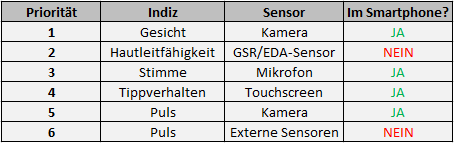
\includegraphics[width=16cm]{Bilder/prio.png}
	\caption[Priorisierung der Erfassungsmöglichkeiten]{Priorisierung der Erfassungsmöglichkeiten}
\end{table}%
\newline In der ersten Spalte ist die Priorität dargestellt. Je niedriger die Zahl ist, desto höher ist die Erfassungsmöglichkeit priorisiert. Die Möglichkeiten werden in der Reihenfolge der hier dargestellten Priorisierung thematisiert und letzten Endes in den Prototyp der mobilen Applikation integriert, um Daten zu erfassen. Je nachdem wie viel Zeit die einzelnen Features benötigen, können mehr und mehr Möglichkeiten der Datenerfassung in die App eingebaut werden, wenn sie noch im Zeitrahmen der Studienarbeit umsetzbar sind. Bei den einzelnen Möglichkeiten werden das Indiz, anhand dessen Rückschlüsse auf eine Emotion gemacht werden kann, und ein Sensor, der Daten zum Indiz für die App erfassen soll, aufgelistet. In der letzen Spalte ist festgehalten, ob der benötigte Sensor in den meisten aktuellen Smartphones bereits enthalten ist oder nicht. \newline
Die höchste Priorität hat die Erfassung des Gesichts mit der Smartphone-Kamera. Grund hierfür ist, dass die Gesichtserkennung sehr genaue Rückschlüsse auf die Emotionen zulässt. Die Ergebnisse liefern außerdem Hinweise für viele unterschiedliche Emotionen, aus welchem Grund die Gesichtserkennung eine gute Basis für die Emotionsbestimmung der mobilen Applikation darstellt. Zusätzliche Indizien können die Ergebnisse der Gesichtserkennung verstärken oder relativieren. Des Weiteren ist vorteilhaft, dass die Erfassungsmöglichkeit ohne externe Sensoren auskommt und lediglich die Smartphone-Kamera genutzt werden kann. 
\newline
Die nächst höhere Priorität hat das Indiz der Hautleitfähigkeit, das mithilfe von GSR- beziehungsweise EDA-Sensoren erfasst werden kann. Diese Art von Sensoren befinden sich wie bereits beschrieben nicht in handelsüblichen Smartphones, weshalb man hierzu einen Arduino verwenden muss, der anschließend Daten an die App weiterleitet. Obwohl dies ein Nachteil ist, wurde diese Erfassungsmöglichkeit so hoch priorisiert, da dies ein Bereich in der App-Entwicklung ist, der nur selten thematisiert wird. Dieses Potenzial ist zusammen mit Aussagekraft der Aktivation zu bestimmten Emotionen der Hauptgrund für die hohe Priorisierung. Jedoch muss die Messung der Hautleitfähigkeit mit einem anderen Erfassungstest kombiniert werden, da die Messung alleine keine eindeutigen Anzeichen für einzelne Emotionen zurückliefert, sondern für mehrere.\newline
An dritter Stelle steht die Stimmerkennung mithilfe des Smartphone-Mikrofons. Obwohl aus der Stimme auch viele Anzeichen für Emotionen herausgelesen werden können und ein Mikrofon in jedem Smartphone integriert ist, hat die Stimmerkennung einen Nachteil. Der Benutzer müsste dazu über eine längeren Zeitraum in das Mikrofon sprechen. Da er das für eine Durchführung der Messung zwingend machen muss, besteht auch die Gefahr, dass die Stimme des User nicht natürlich ist, sondern aufgesetzt ist, da er sich über die Durchführung des Test bewusst ist. Da mit der Gesichtserkennung außerdem bereits eine umfangreiche Basis für die Emotionsbestimmung vorhanden ist, erfolgt die Priorisierung auf Platz 3. \newline
Auf dem vierten Platz folgt die Erfassung des Tippverhaltens mit dem Touchscreen beziehungsweise mit der eingeblendeten Tastatur des Smartphones. Hier ist der selbe Nachteil vorhanden wie bei der Stimmerkennung. Der User muss über eine längere Zeit Eingaben über den Touchscreen vornehmen und er ist sich nach Start des Tests bewusst, dass seine Eingaben analysiert werden. Deshalb ist das Ergebnis des Tippverhaltens-Test einfach manipulierbar. Außerdem ist es auch bezüglich der Privatsphäre des Users problematisch, seine eingegebenen Texte zu analysieren. Trotzdem können bei ehrlicher, nicht manipulierter Benutzung des Test interessante Ergebnisse für die Emotionsbestimmung gewonnen werden. \newline
Auf Platz 5 und 6 folgt die Pulsmessung. Da die meisten Erkenntnisse, die mit der Messung des Puls bezüglich Emotionen gewonnen werden können, bereits mit der Hautleitfähigkeits-Messung abgedeckt werden, sind diese beiden Möglichkeit niedrig priorisiert. Die Pulsmessungen können im besten Fall die Ergebnisse des GSR-Sensor bekräftigen, liefern aber neue keine neuen Erkenntnisse. Die Messung mit der integrierten Smartphone-Kamera wird trotz der vermeindlich geringeren Genauigkeit höher priorisiert als die Messung mit dem externen Arduino-Sensor, da dort keine zusätzliche Hardware verwendet werden muss. \newline
Auf den letzten Platz liegt die Messung der Gangart. Obwohl es sich hierbei auch eine Messung biometrischer Daten handelt, können hieraus nur sehr wenige Anzeichen für Emotionen herausgelesen werden. Von allen beschriebenen Methoden liefert diese Möglichkeit den geringsten Nutzwert für die Zwecke der mobilen Applikation. Aus diesem Grund hat die Implementierung dieser Messung die geringste Priorität. \newline
% Zu diskutieren: Eigentlich wäre Reihenfolge Gesicht, GSR, Stimme, Tippverhalten sinnvoller, da im Theorieteil sich herausstellt das nur mit dem Gesicht ein direkter Schluss auf Emotionen möglich ist. 
\subsection{Übertragung biometrischer Daten in Indikatorscores}
\subsectionauthorlong{Lukas Seemann}
Die von den Smartphone-internen und externen Sensoren zurückgeliefert Daten müssen in der App einheitlich verarbeitet werden. Die zurückgelieferten Daten sind unterschiedlich und meistens selbst nicht aussagend. Mit dem im Theorieteil erklärten Hintergrundwissen ist es jedoch möglich, die Daten zu interpretieren. \newline 
Im Umfeld der App soll diese Interpretation mithilfe von Indikatoren geschehen. Ein Indikator ist in diesem Kontext ein Anzeichen, das für die Emotionsbestimmung herangezogen werden kann. Es existieren einerseits Indikatoren, die sich nur für die Bestimmung einer Emotion eignen, und andererseits auch Indikatoren, die für mehrere Emotionen ausschlaggebend sind. Folgende Indikatoren sind für die Umsetzung geplant: 
\begin{itemize}[noitemsep, topsep=0pt]
	\item activation,
	\item happyIndicator,
	\item sadIndicator,
    \item angryIndicator und
    \item suprisedIndicator.
\end{itemize}
\begin{figure}[h]
	\centering
	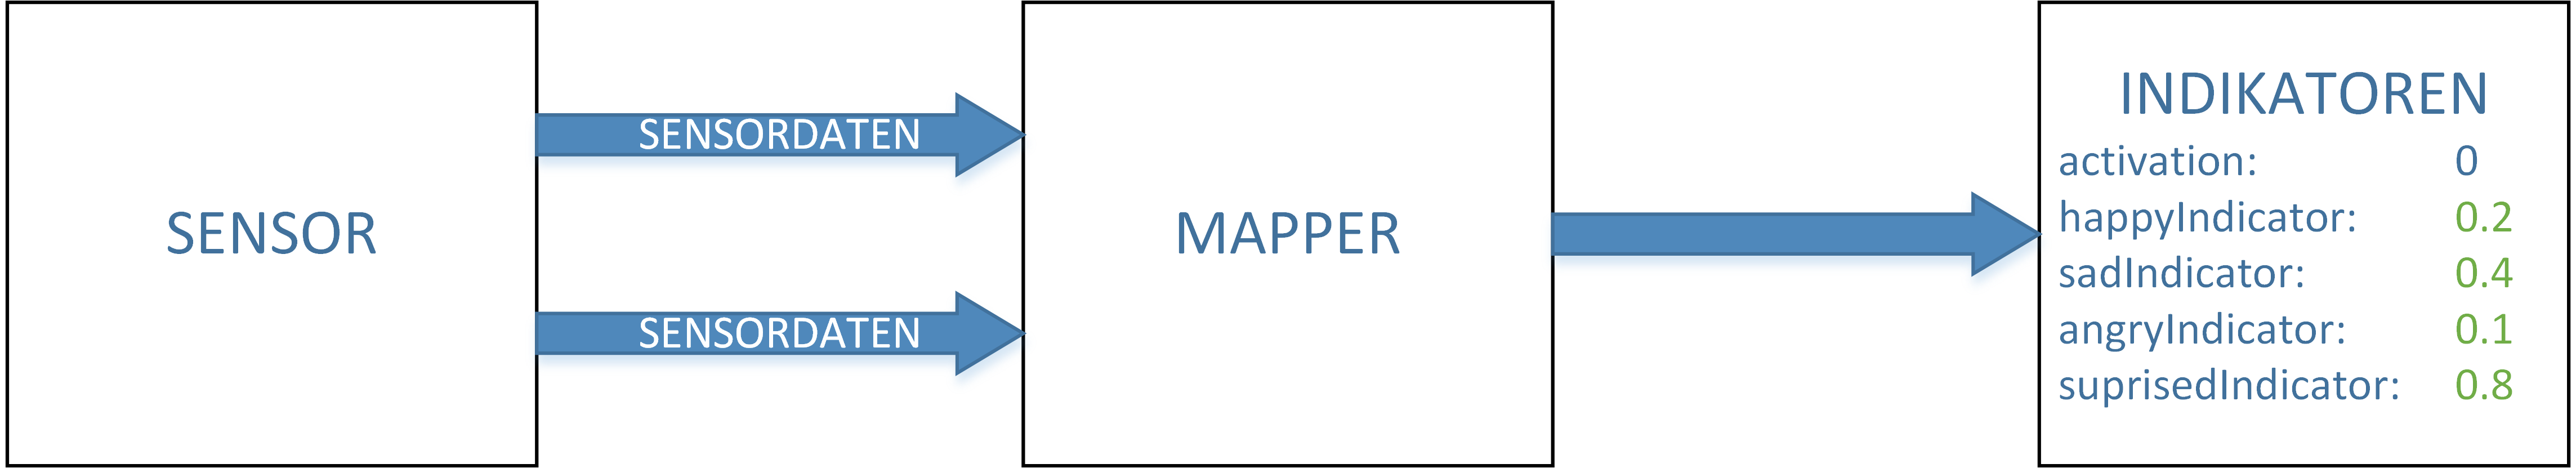
\includegraphics[width=16cm]{Bilder/indicatorscore.png}
	\label{img:Ablauf Erstellung Indicatorscores}
	\caption[Ablauf der Erstellung von Indikatorscores]{Ablauf der Erstellung von Indikatorscores}
\end{figure}%
In Abbildung ? ist der Ablauf der Bestimmung von Indikatorscores abbgebildet. Unabängig davon, welcher Sensor verwendet wird, seine Daten müssen immer auf diese Indikatoren abgebildet werden. Für jeden Sensor muss dabei ein Bereich bestimmt werden, wann immer eine neue Auswertung der Sensordaten zu den sogenannten Indikatorscores geschieht. Eine Auswertung kann generell dann durchgeführt werden, wenn genug Daten vorhanden sind, die aussagekräftig für die Indikatoren sind. Dies ist von Sensor zu Sensor unterschiedlich und muss dementsprechend berücksichitgt werden. \newline
Bei einer Auswertung werden die einzelnen Indikatoren mit Scores von null bis eins versehen, sodass man pro Auswertung der Sensordaten mehrere Indikatorscores erhält. Die Logik für das Setzen der Indikatorscores muss mithilfe von Mappern umgesetzt werden. Für jeden Sensor muss dafür ein individueller Mapper existieren. Die Mapper werden immer dann aufgerufen, wenn genügend Daten des Sensors vorhanden sind. \newline
\subsection{Auswertung der Indikatorscores zur Emotionsbestimmung}
\subsectionauthorlong{Lukas Seemann}
Aus den angesammelten Indikatorscores muss nun entschieden werden, welche Emotion am wahrscheinlichsten beim Benutzer der App vorliegt. Diese Auswertung der Indikatorscores zu konkreten Emotionen erfolgt mit einer Menge von Kausalitätsregeln. Als Ergebnis wird pro Emotion ein Emotionscore erwartet, der angibt, inwiefern die Emotion beim User zum getesteten Zeitpunkt vorliegt. Anschließend muss geplant werden, in welchem zeitlichen Abstand ein neue Emotionscores angelegt werden.
\subsubsection{Kausalitätsregeln}
\subsubsectionauthor{Lukas Seemann}
Eine Kausalitätsregel erwartet eine Menge von Indikatorscores als Eingabe und wendet basierend auf den Indikatorscores Effekte auf die vorhandenen Emotionscores an. Die Indikatoren werden also je nach ihren Werten in verschiedene Emotionen übersetzt. \newline Eine Kausalitätsregel besteht immer aus einer Bedingung und einer Score-Transformation. Eine Bedingung betrifft einen oder maximal zwei Indikatorscores und legt fest, wann die Score-Transformation der Kausalitätsregel ausgeführt wird. Die Score-Transformation beschreibt Effekte, die auf die Emotionscores angewandt werden. Beispielsweise würde einer hoher Score des Stress-Indikators zu positiven Effekten für die Emotionen happy, angry und suprised führen. In Abbildung ? ist der Ablauf der Ausführung einer solchen Kausalitätsregeln gezeigt. Die Formulierung von realitätsgetreuen Kausalitätsregeln ist ausschlaggebend dafür, wie präzise die Anwendung letzten Endes die Emotionen bestimmmen kann. \newline
\begin{figure}[h]
	\centering
	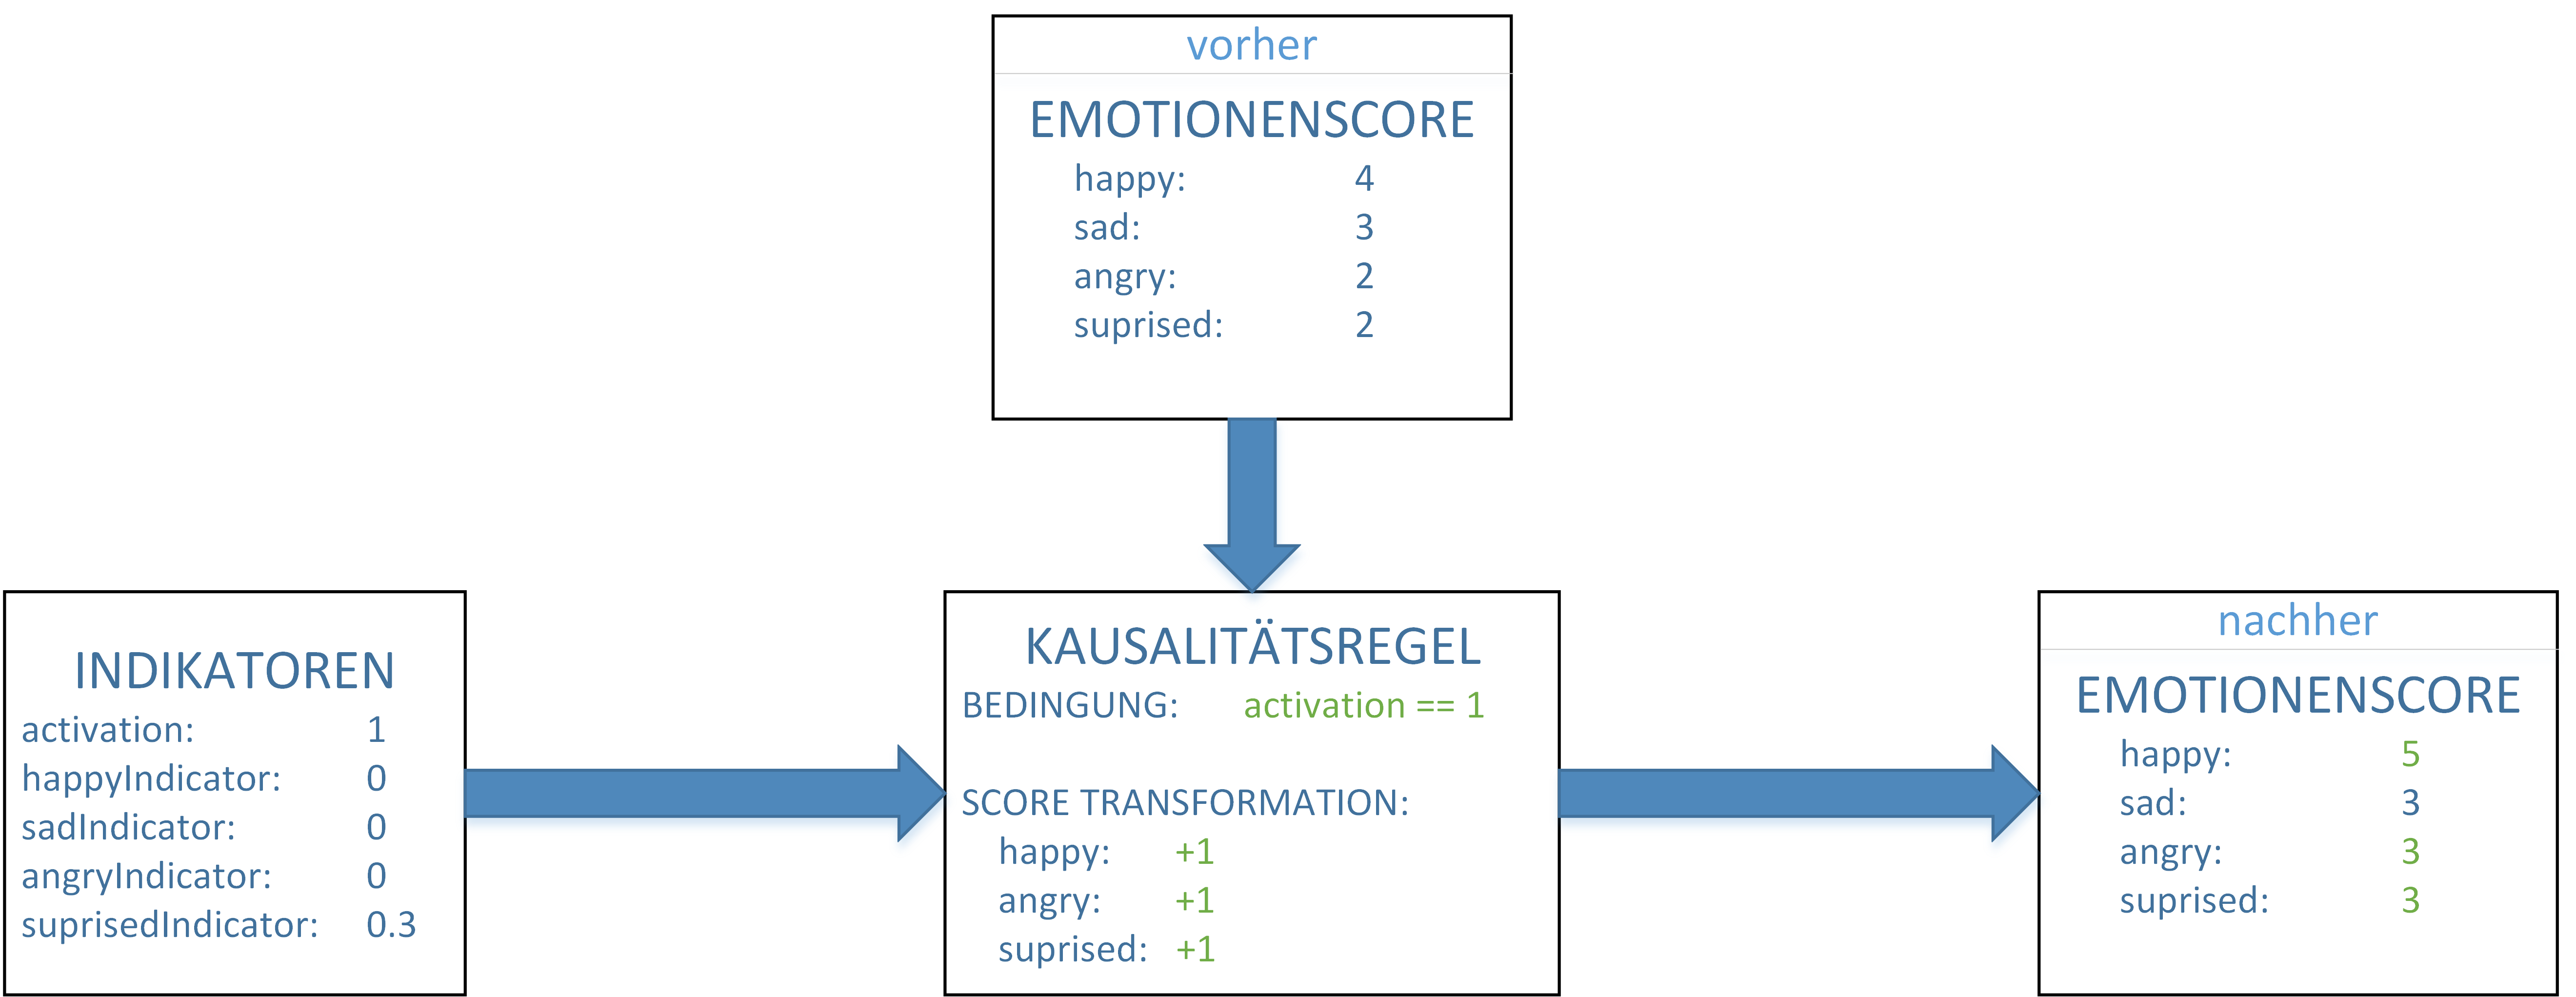
\includegraphics[width=16cm]{Bilder/causalityrules.png}
	\caption[Ablauf der Ausführung von Kausalitätsregeln]{Ablauf der Ausführung von Kausalitätsregeln}
\end{figure}%
\subsubsection{Unterteilung der Entscheidung in Intervalle}
\subsubsectionauthor{Lukas Seemann}
Es wurde bereits beschrieben, wie aus Sensordaten Indikatorscores gewonnen werden und wie wiederum aus diesen mithilfe der Kausalitätsregeln Emotionscores ermittelt werden. Nun muss bestimmt werden, wie oft jeweils neue Emotionscores erstellt und eine Anwendung der Kausalitätsregeln durchgeführt wird. \newline
Um später einen zeitlichen Ablauf der Emotionen des Nutzern anzeigen zu können, muss ein minimaler Zeitbereich bestimmt werden, für den die Auswertung in Emotionscores durchgeführt werden kann. Angedacht ist hierbei, dass der User alle 10 Sekunden ein neue Auswertung erhält. Folglich bedeutet das, dass alle IndicatorScores die in einem 10-Sekunden-Intervall registriert wurden, zusammengefasst werden und für diese dann alle Kausalitätsregeln durchgeführt werden. Dies bedeutet das alle 10 Sekunden ein neue Emotionscores erzeugt werden und anhand der im Intervall vorhandenen Indikatorscores verädert werden. So wird dem User ermöglicht, alle 10 Sekunden eine Bestimmung seiner Emotion in diesem Intervall zu erhalten.
\subsection{Ionic Framework}
In diesem Kapitel wird das Ionic Framework, das für die Umsetzung der mobilen Applikation verwendet wird, vorgestellt und die Gründe für die Verwendung aufgezeigt.
\subsubsection{Aufbau und Einsatz des Frameworks}
\subsubsectionauthor{Lukas Seemann}
Ionic ist ein unter der MIT License stehendes Open-Source-Framework, das zur Entwicklung von plattformübergreifenden, mobilen Applikationen dient. Mit Ionic entwickelte Apps sind damit unter anderem auf Endgeräten lauffähig, die die Betriebssysteme Android, iOS und Windows Phone benutzen. \footcite{Ion18a}
\begin{figure}[h]
	\centering
	
\includegraphics[width=11cm]{Bilder/ionic.png}
	\caption[Ionic Framework - Logo]{Ionic Framework - Logo\footnotemark}
\end{figure}%
\footcitetext{Wik18}
\newline
Aktuell befindet sich das Framework in der Version 3.9.2\footcite[Vgl. ][]{Ion18b} und befindet sich in stetiger Weiterentwicklung. Das Ionic Framework basiert wiederum auf Angular, einem Framework für die Entwicklung von Web-Applikationen. Dementsprechend nutzen Ionic-Anwendungen in der Web-Entwicklung etablierte Technologien wie HTML 5, CSS und JavaScript. \footcite[Vgl. ][]{Ion18c} Wie auch im Angular Framework, wird auch die Programmiersprache TypeScript verwendet, die auf JavaScript aufbaut, sich in der Syntax sehr stark mit JavaScript ähnelt und zusätzliche Optionen zur Typisierung von Variablen oder Funktionen anbietet. \footcite[Vgl. ][]{Til17} \newline
Ionic-Anwendungen sind im Wesentlichen normale Webanwendungen, die von jedem JavaScript-fähigen Browser ausgeführt werden können. Während mithilfe von Ionic das Frontend der Anwendung festgelegt wird, kann anschließend mit Apache Cordova die Plattformunabhängigkeit umgesetzt werden. Apache Cordova bewirkt, dass sich die Webanwendungen wie native Android-, iOS- oder Windows Phone-Applikationen anfühlen. Egal auf welcher Plattform die Ionic-Anwendung installiert wird, es wird die selbe Code-Basis verwendet. Diese wird dann vor dem Installieren von Cordova so angepasst, dass sie auf den Endgeräten ausgeführt werden können. \footcite{Ion18d}
\subsubsection{Gründe für die Verwendung}
\subsubsectionauthor{Lukas Seemann}
Das Ionic Framework bietet eine Möglichkeit mit nur einer Code-Basis, eine plattform-übergreifende Applikation zu erstellen. Dies erspart einiges an Entwicklungsaufwand, da nicht jede Plattform einzeln entwickelt werden muss. Außerdem wird einem Großteil der Smartphone-Nutzer die Nutzung der erstellten App ermöglicht und ist nicht nur für Android- oder Apple-Nutzer beschränkt. \newline
Dadurch dass Applikationen des Ionic Frameworks eigenständige Webanwendungen sind, können diese problemlos von allen Browsern interpretiert und ausgeführt. Dies ist ein großer Vorteil für das Debuggen von Code, da hierfür kein Emulator oder Endgerät verwendet werden muss. Stattdessen kann die Anwendung im Browser ausgeführt und debuggt werden. \newline
Außerdem wurden bereits in anderen Projekten und im privaten Bereiche Erfahrungen mit dem Ionic Framework gemacht, sodass keine Einarbeitung bei den Entwicklungsarbeiten notwendig ist. Dies spart wiederum Zeit, die effektiv für das Entwickeln genutzt werden kann. 
\subsection{Architektur der mobilen Applikation}
In diesem Kapitel wird die Architektur der mobilen Applikation beschrieben. Die Architektur wird in Front- und Backend der App unterteilt.
\subsubsection{Backendlogik}
\subsubsectionauthor{Lukas Seemann}
Zunächst wird explizit auf das Backend beziehungsweise die Hintergrundlogik der App eingegangen. Für das oben beschriebene Konzept bietet sich eine Umsetzung mit Javascript Klassen an, aus welchem Grund ein UML-Diagramm angefertigt werden kann. Dieses ist in Abbildung ? gezeigt. \newline
\begin{figure}[h]
	\centering
	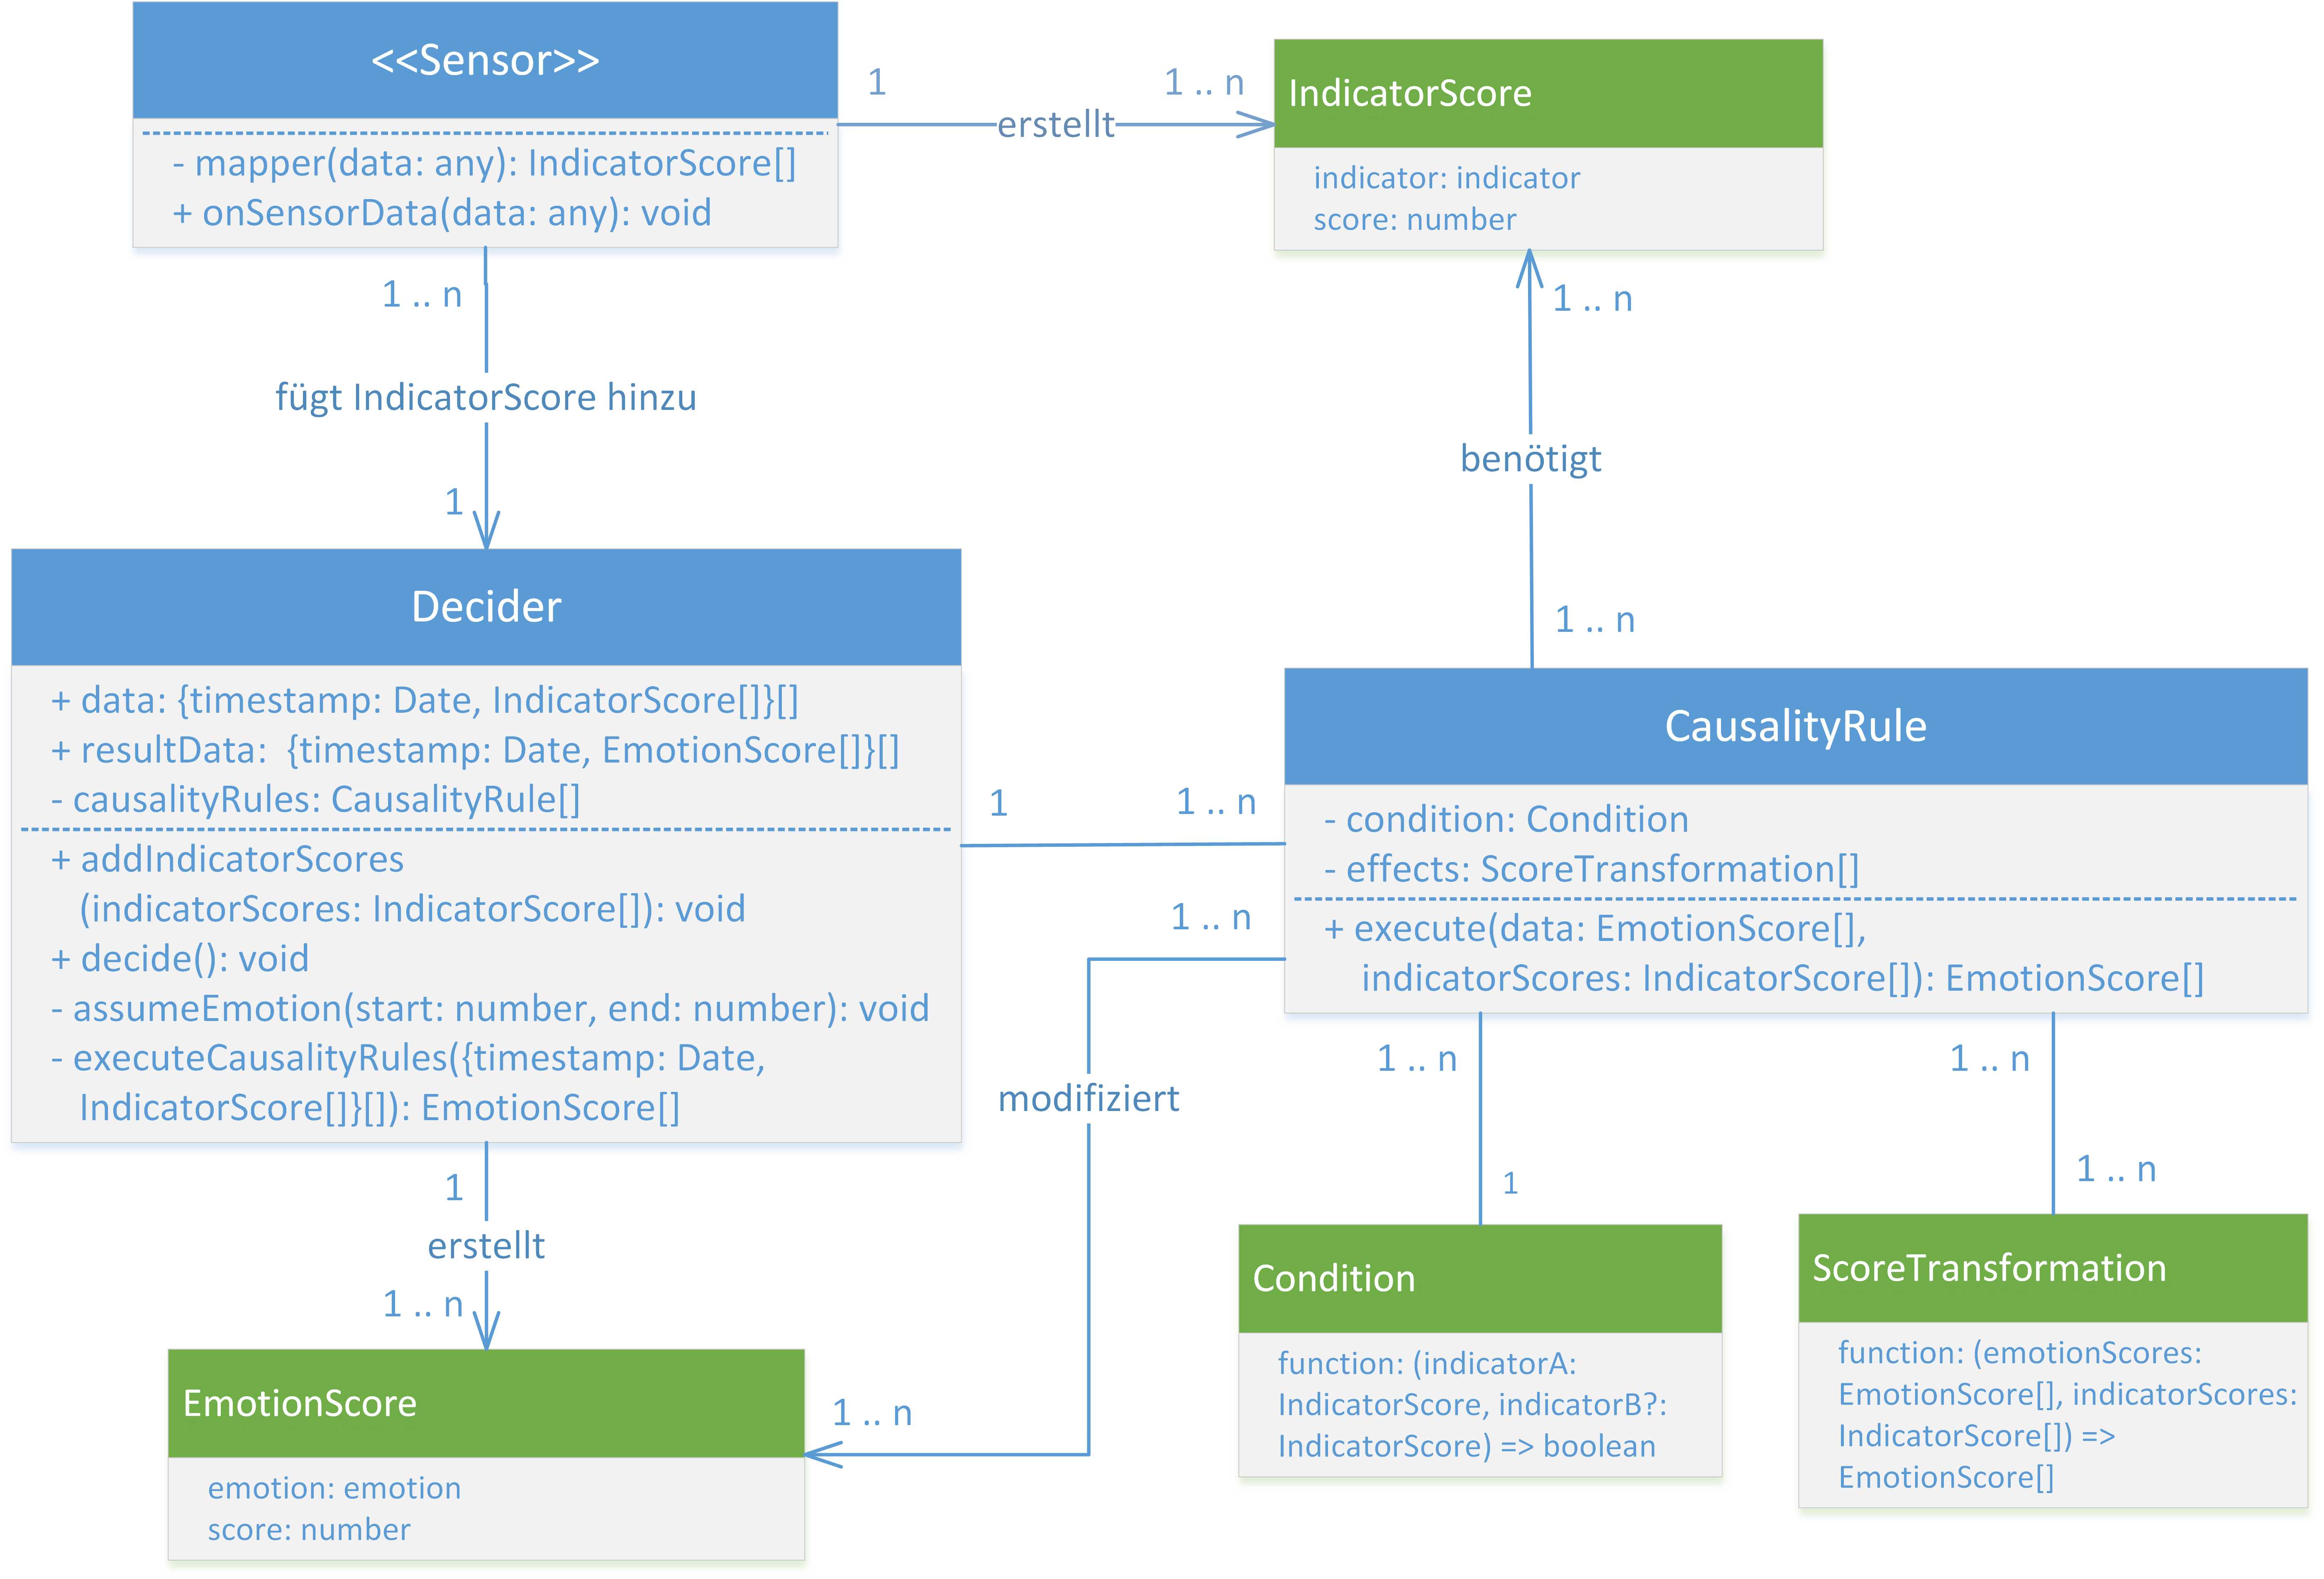
\includegraphics[width=16cm]{Bilder/architecture.png}
	\caption[Architektur der App]{Architektur der App}
\end{figure}%
\newline
Die Klassen sind in der Abbildung blau dargestellt. Typescript bietet die Möglichkeit, eigene Typen zu definieren. Diese Typen verfügen über Attribute, jedoch keine Methoden und sind in der Abbildung grün dargestellt. \newline 
Die App verfügt über eine abstrakte Klasse Sensor, die zwei Methoden definiert. Jeder Sensor, der später Daten für die App liefern soll, muss diese abstrakte Sensor-Klasse erweitern. Dabei muss jeder Sensor die mapper-Funktion überschreiben, die die Sensordaten in mehrere IndicatorScores umwandelt. Auf diese Weise muss jeder Sensor seinen individuellen Mapper implementieren. Der IndicatorScore ist als Typ definiert worden, der einerseits einen Indicator und einen Score als Attribut hat. Indicator wiederum ist ein eigener Typ, der nur die definierten Indikatoren (stress, happyIndicator, sadIndicator, angryIndicator, suprisedIndicator) als String zulässt. Da die Implementierung des IndicatorScore-Types sehr trivial ist, wurde sie aus Übersichtsgründen nicht in die Abbildung aufgenommen. Die onSensorData-Funktion ist bereits vordefiniert und muss dementsprechdend nicht überschrieben werden. Diese Funktion führt lediglich den Mapper aus, wenn genug Sensordaten für eine Auswertung vorhanden sind, und fügt die resultierenden IndicatorScores zum Decider hinzu. \newline \newline
Die Decider-Klasse ist der Hauptbestandteil der App, da sie die Bestimmung der Emotion durchführt. Die Decider-Klasse ist als Singleton anzusehen, da es pro laufende Anwendung nur einen Decider geben kann. Der Decider verfügt über ein data-Array, das allen Input der Sensoren enthält. Konkret handelt es sich hierbei um die Indicatorscores, die die Sensoren ermittelt haben, erweitert mit einem Timestamp für den Zeitpunkt der Ankunft. Nach und nach wird dieses Array mit den IndicatorScores der verschiedenen Sensoren gefüllt. Dies wird mit der Funktion addIndicatorScores() realisiert, die von den Sensoren mit der onSensorData-Funktion aufgerufen wird. \newline
Der Decider verfügt außerdem über ein Array von CausalityRules. Die CausalityRule-Klasse ist die Implementierung der oben beschriebenen Kausalitätsregel. Eine CausalityRule besitzt immer eine Condition (Bedingung) und eine Menge von ScoreTransformationen. \newline
Eine Condition wurde als eigener Typ definiert und ist eine Funktionen, die einen  IndicatorScore (optional auch zwei) als Input hat und auf einen Boolean-Wert abbildet. So kann eine Bedingung realisiert werden, die je nach Erfüllung true oder false zurückgibt. Eine ScoreTransformation ist ebenfalls ein eigener Typ, der eine Funktion definiert. Diese Funktion erhält als Input die vorhandenen Emotionscores, wendet auf diesen Effekte an und gibt die modifizierten Emotionscores zurück. \newline
Die execute-Funktion der CausalityRule führt alle hinterlegten ScoreTransformations aus, wenn die Condition von den IndicatorScores erfüllt worden ist. \newline
Um die Decider-Klasse weiter zu verstehen, muss zunächst der Typ Emotionscore erklärt werden. Dieser ist ähnlich wie der IndicatorScore aufgebaut. Zunächst wird eine Emotion angegeben, die dem Typ Emotion entsprechen muss. Der String muss dementsprechend mit den definierten Emotionen (happy, sad, angry, suprised) übereinstimmen. Anschließend folgt eine Nummer, die den Score angibt.\newline \newline
Die Decider hat ein resultData-Array, das mehrere Emotionscores enthält und die Timestamp der IndicatorScores, aus denen die Emotionscores erzeugt wurden. Dieses Array wird mithilfe der decide-Funktion gefüllt. Wenn die decide-Funktion ausgeführt wird, wird anschließend für alle im data-Array vorhandenen Timestamps die assumeEmotion()-Funktion ausgeführt. Als Parameter erhält diese Methode eine Timestamp und filtert alle IndicatorScores aus dem data-Array zu diesem Zeitpunkt. Für alle auf diese Weise gefilterten Indicatorscores wird anschließend die executeCausalityRules()-Funktion ausgeführt. Diese Funktion wiederum iteriert über alle vorhandenen CausalityRules und führt diese auf Basis der IndicatorScores aus. So erhält man am Ende Emotionscores. Diese erhalten die Timestamp, die bei assumeEmotion() mitgegeben wurde und werden in das resultData-Array gespeichert. Hat man die assumeEmotion-Funktion für alle Timestamps ausgeführt, ist das result-Array komplett gefüllt und die Emotionsbestimmung abgeschlossen.
\subsubsection{Frontend}
\subsubsectionauthor{Lukas Seemann}
Nachdem bereits das Backend beschrieben wurde, wird nun das Frontend der App thematisiert. Unter dem Frontend werden die Screens der App verstanden, die der User bei Nutzung der App aufrufen kann. Diese Screens werden bei Ionic Pages genannt und bestehen meist aus folgenden Bestandteilen: 
\begin{itemize}[noitemsep, topsep=0pt]
	\item Eine Typescript-Datei (.ts), 
	\item eine HTML-Datei (.html) und
	\item eine CSS-Datei (.scss).
\end{itemize}
In der Typescript-Datei wird die Anwendungslogik umgesetzt, außerdem erfolgt dort der Zugriff auf die Backendkomponenten wie zum Beispiel den Decider, die durch das Ionic Framework als sogenannte Provider bereitgestellt werden. Die HTML-Datei beschreibt den Aufbau der GUI der Page, wohingegen die CSS-Datei das Design der Page beschreibt. \newline
In Abbildung ? ist zu sehen, über welche Pages die App verfügen soll, welchen Zweck diese haben und wie sie miteinander in Verbindung stehen.
\begin{figure}[h]
	\centering
	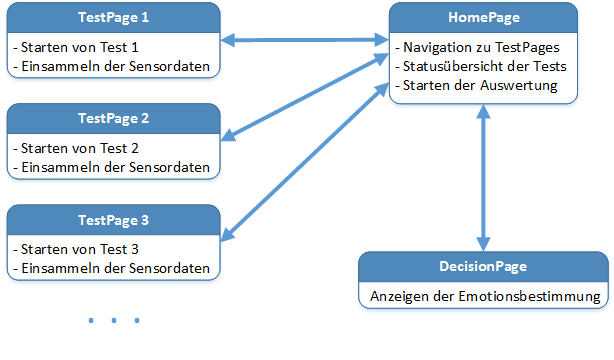
\includegraphics[width=15cm]{Bilder/frontend.png}
	\caption[Geplantes Frontend der App]{Geplantes Frontend der App}
\end{figure}% 
\newline
Für die App sollen nach und nach sogenannte Emotionstest entwickelt werden. Unter einem Emotionstest versteht man im Kontext dieses Projekts die Messung eines Sensors, die Rückschlüsse auf die Emotion zulassen. Ein Emotionstest liefert aus Backend-Sicht immer eine Menge von Indikatorscores zurück. Pro Emotionstest muss eine Page der App angelegt werden, auf der der Test gestartet werden kann und so die Sensormessdaten eingesammelt werden können. \newline
Zwangsläufig verfügt die App über eine HomePage, auf die der User beim Starten der App gelangt. Über diesen Screen kann der User zu den einzelnen TestPages gelangen, um die Tests durchzuführen. Von den TestPages kann der User entweder durch Abschließen der Tests oder durch manuelles Navigieren und Unterbrechen des Test zurück zum Homescreen gelangen. Um dem User anzuzeigen, welche Test er schon durchgeführt hat, wird außerdem eine Statusübersicht zu den Tests auf der HomePage zu sehen sein. Des Weiteren muss der User die Möglichkeit haben, die Auswertung der Indicatorscores zu Emotionen starten zu können. Wählt der User diese Option, werden alle Indicatorscores, die sich zu diesem Zeitpunkt im data-Array des Deciders befinden für die Auswertung verwendet. \newline
Für das Ergebnis der Auswertung und somit die Emotionsbestimmung muss ebenfalls eine eigene Page existieren, worauf der User nach Abschluss der Auswertung gelangt. Der User kann von diesem Screen wieder zurück zum Homescreen gelangen, um erneut Emotionstests zu starten. 
\subsubsection{Vor- und Nachteile der Architektur} 
\subsubsectionauthor{Lukas Seemann}
In diesem Abschnitt werden die Vor- und Nachteile der vorgestellten Architektur gegenübergestellt werden. \newline
Ein Vorteil der Architektur ist es, dass beliebige viele Sensoren und somit Emotionstest hinzugefügt werden können, ohne dass das Backend abgeändert werden müsste. Neue Sensoren müssen lediglich, dass Sensor-Interface implementieren und folglich die mapper-Funktion überschreiben. So kann die App in Zukunft beliebig erweitert werden. \newline
Ein weiterer Vorteil ist, dass die Auswertung der IndicatorScores zu Emotionscores zentral über die Kausalitätsregeln verwaltet werden kann, deren Aufbau bereits vorgegeben ist. Da die Kausalitätsregeln ausschlaggebend für die Emotionsbestimmung sind, müssen diese bei Bedarf angepasst werden, wenn Endergebnisse der Emotionsbestimmunf nicht passend sind. Diese Anpassung kann zentral im Array der Kausalitätsregeln geschehen, und es müssen keine Funktionen umgeschrieben werden oder die Architektur abgeändert werden. \newline
Des Weiteren hat die Aufteilung in IndicatorScores und Emotionscores den Vorteil, dass im gesamten Backend eine einheitliche Datengrundlage vorliegt. Da verschiedene Sensoren ganz unterschiedliche Daten zurückliefern, müssen diese vereinheitlicht werden. Dies wurde mithilfe der IndicatorScores und der EmotionScores umgesetzt. Alle Sensoren, die in Zukunft hinzugefügt werden, müssen sich an die Datenstruktur dieser Scores anpassen. Dies wird durch die Mapper und Kausalitätsregeln sichergestellt. \newline
\newline
Ein Nachteil der Architektur ist, dass eine Anpassung der IndicatorScores und der Emotionscores Änderungen an vielen Stellen hervorrufen würde. Will man beispielsweise einen neuen Indikator \textit{disgustIndicator} und eine neue Emotion \textit{disgust} hinzufügen, müssen zunächst alle Funktionen des Deciders angepasst werden, damit diese neue Emotion aufgenommen werden kann. Des Weiteren müssen gegebenenfalls viele vorhandenen Mapper und Kausalitätsregeln angepasst werden, da diese den neuen Indikator beziehungsweise die neue Emotion nicht berücksichtigt haben.
\subsection{MockUps}
\subsectionauthor{Torben Brenner}
Bevor wir mit der Arbeit an dem Prototypen begonnen haben, diskutierten wir zuerst das Design der einzelnen Komponenten der Anwendung. Wir einigten uns darauf, dass die Übersicht über alle Teile des Prototypen auf der Hauptseite des Startbildschirms sein soll (siehe \ref{img:Mockup-Home}).
\begin{figure}[h]
	\centering
	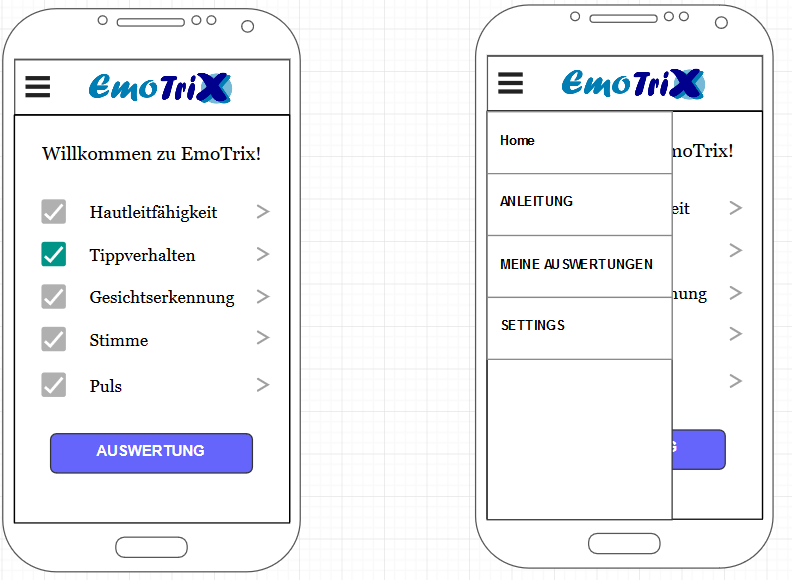
\includegraphics[width=10cm]{Bilder/Mockup-Home.png}
	\label{img:Mockup-Home}
	\caption[Mockup - Homescreen(links) und Menü(rechts)]{Mockup - Homescreen(links) und Menü(rechts)}
\end{figure}%
Wie auf der Grafik zu sehen ist, sind für die fertige Anwendung 5 verschiedene Arten von Tests vorgesehen. Die dazugehörigen Anwendungsabschnitte sollen von der Startseite, durch anklicken des Testnamens aufgerufen werden können und dann ausgeführt werden können. Durch das Berühren des Auswertungsknopfes soll es möglich sein, eine Analyse der verschiedenen Testergebnisse durchzuführen. Diese gibt dann als Ergebnis eine Übersicht heraus, welche Emotionen wie wahrscheinlich sind. Eine Übersicht der bereits durchgeführten Auswertungen soll über das Menü (siehe \ref{img:Mockup-Home} rechts) erreichbar sein. In der Anleitung(ebenfalls über das Menü erreichbar) sollen sich Beschreibungen zur Durchführung der einzelnen Tests befinden.\newline
Im folgenden soll neben den einzelnen Test Seiten, auch die Auswertungsseite genauer beschrieben werden.
\subsubsection{Hautleitfähigkeit}
\subsubsectionauthor{Torben Brenner}
Der Test der Hautleitfähigkeit benötigt die Verbindung mit dem Arduino Microcontroller. Deshalb muss dem Nutzer die Möglichkeit geboten werden, sich mit diesem über die Software möglichst einfach zu verbinden. Hierzu ist eine Seite für die Verbindung vorgesehen\footnote{zu sehen auf der Abbildung Mockup - Arduino verbinden}. 
\begin{figure}[h]
	\centering
	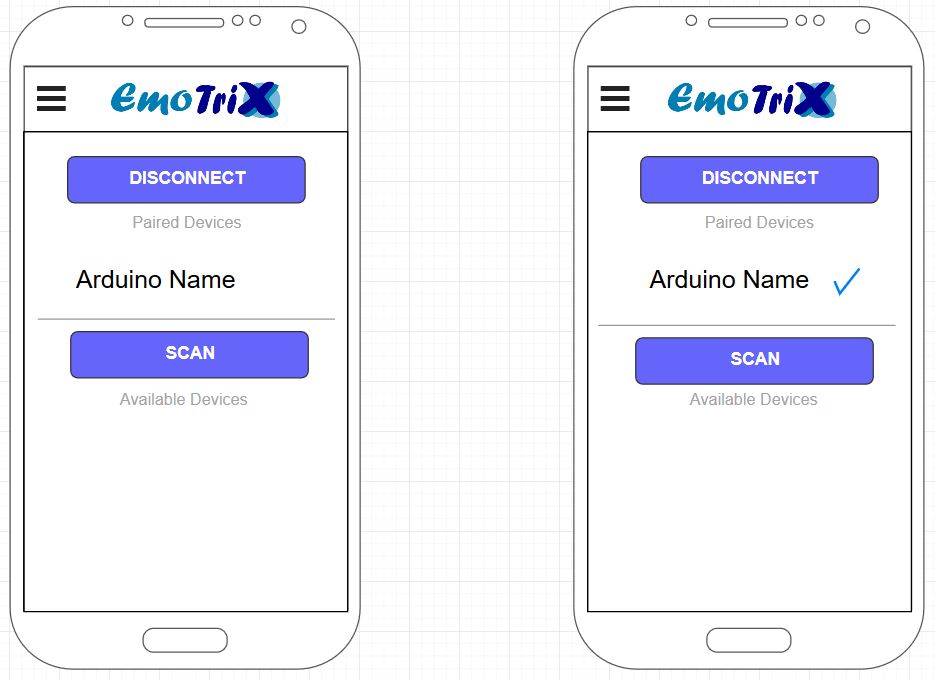
\includegraphics[width=10cm]{Bilder/Mockup-Arduino-Connection.png}
	\label{img:Mockup-Arduino-Connection}
	\caption[Mockup - Arduino verbinden(links nicht verbunden, rechts verbunden)]{Mockup - Arduino verbinden(links nicht verbunden, rechts verbunden)}
\end{figure}%
Auf dieser Seite hat der Nutzer die Möglichkeit, nach verfügbaren Geräten zu suchen. Da der Arduino mittels Bluetooth verbunden wird, werden in der Liste der verfügbaren Geräte auch andere Bluetoothgeräte angezeigt. Bei der Auswahl eines Gerätes wird versucht eine Verbindung mit diesem aufzubauen. Ist dieser Versuch erfolgreich, wird der Name des Gerätes zusammen mit einem Hacken dargestellt. Beim öffnen der Seite ist es ebenfalls möglich, dass der Name des Arduino bereits angezeigt wird. In diesem Fall soll es möglich sein, den Namen zu berühren um eine Verbindung aufzubauen. Gelingt diese wird ebenfalls ein Hacken hinter den Namen gesetzt.\newline
Wo die Verbindung mit dem genau durchgeführt wird, ist noch nicht festgelegt. Denkbar wäre zum einen eine Settingsseite von der aus diese Einstellung erreichbar wäre, zum anderen ist es auch möglich, dass diese Seite angezeigt wird sobald der Test aufgerufen wird.\newline
Der Test ist folgendermaßen aufgebaut. Der Nutzer schließt sich extern an den Hautleitfähigkeitssensor an. Hier sollte die Anleitung genauere Details enthalten wie das zu bewerkstelligen ist. Wenn der Nutzer an den Hautleitfähigkeitssensor angeschlossen ist und mit dem Arduino verbunden ist, kann der Test gestartet werden. Die Messungen beginnen nach dem drücken des Startknopfes. Danach sendet der Sensor über Bluetooth die Daten, welche in Form eines Graphen auf der Oberfläche dargestellt werden\footnote{siehe Abbildung \textit{Mockup - Hautleitfähigkeit Test} auf S.\pageref{img:Mockup-GSR}}. 
\begin{figure}[h]
	\centering
	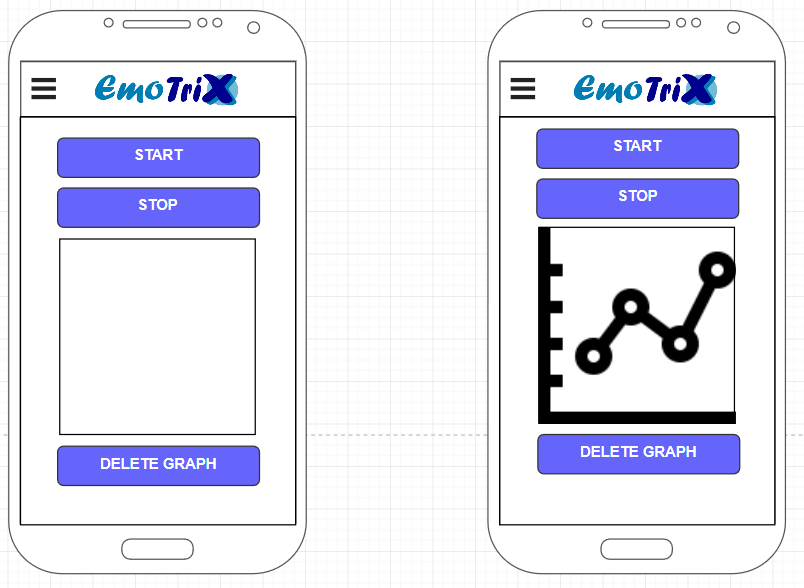
\includegraphics[width=10cm]{Bilder/Mockup-GSR.png}
	\label{img:Mockup-GSR}
	\caption[Mockup - Hautleitfähigkeit Test starten(links) und Test Ergebnis(rechts)]{Mockup - Hautleitfähigkeit Test starten(links) und Test Ergebnis(rechts)}
\end{figure}%
Auf der Seite direkt werden keine Auswertungen der Emotionen dargestellt, sondern nur die Daten des Sensors. Durch betätigen des Stopknopfes, soll die Messung gestopt werden. Mit dem Knopf ``DELETE GRAPH'' wird der gezeichnete Graph zurückgesetzt, aber nicht die bisher erfassten Daten.
\subsubsection{Tippverhalten}
\subsubsectionauthor{Torben Brenner}
Beim Test des Tippverhaltens, ist es angedacht das der Nutzer mit einem ChatBot kommuniziert und die Anwendung im Hintergrund bei Nutzereingaben das Tippverhalten überprüft. In wie fern die Kommunikation mit dem ChatBot abläuft ist noch nicht ganz klar. Es wäre zum denkbar, dass der ChatBot einfach nur einen Dienst zu Verfügung stellt und somit wenig Interaktion bietet. Interessant wäre auch dass vorbereiten eines bestimmten Gesprächs in dem der Nutzer auch von dem ChatBot provoziert werden könnte.
\begin{figure}[h]
	\centering
	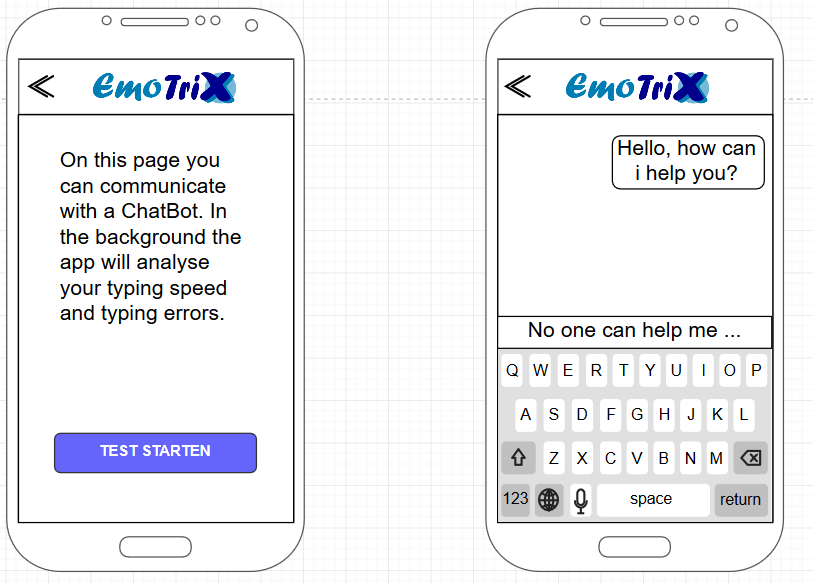
\includegraphics[width=10cm]{Bilder/Mockup-Tippverhalten.png}
	\label{img:Mockup-Tippverhalten}
	\caption[Mockup - Tippverhalten Test starten(links) und Test ergebnis(rechts)]{Mockup - Tippverhalten Test starten(links) und Test ergebnis(rechts)}
\end{figure}% 
Die Oberfläche für die Interaktion mit dem ChatBot soll einem normalen Chat ähneln, d.h. Nachrichten des ChatBots und Antworten des Nutzers werden angezeigt. Der Nutzer bekommt außerdem eine Bildschirmtatstatur angezeigt, auf der er seine Antworten eingeben kann.\newline
Ein Alternative zu diesem Testszenario war, dass der Nutzer einen Zeitraum angibt in dem die App seine Eingaben überwachen darf. Dieser Fall ist aber nicht umsetzbar, da die Betriebssystem natürlich verhindern wollen, dass Passwörter des Nutzers mit gelesen werden können.
Deshalb soll das erste Szenario umgesetzt werden.
\subsubsection{Gesichtserkennung}
\subsubsectionauthor{Torben Brenner}
\label{section:Mockup-Gesichtserkennung}
Bei der Gesichtserkennung wird der Nutzer von der Anwendung dazu aufgefordert, die Kamera zu starten und daraufhin ein Bild mit dieser zu machen. Die Anwendung soll dem Nutzer daraufhin die Aufnahme anzeigen und es ihm ermöglichen das er eine neue Aufnahme machen kann. Wenn der Nutzer eine Aufnahme hat die er analysieren lassen möchte, soll die Anwendung mit Hilfe eines ``Send Picture'' Knopfes die Möglichkeit bieten, dass Bild analysieren zu lassen.
\begin{figure}[h]
	\centering
	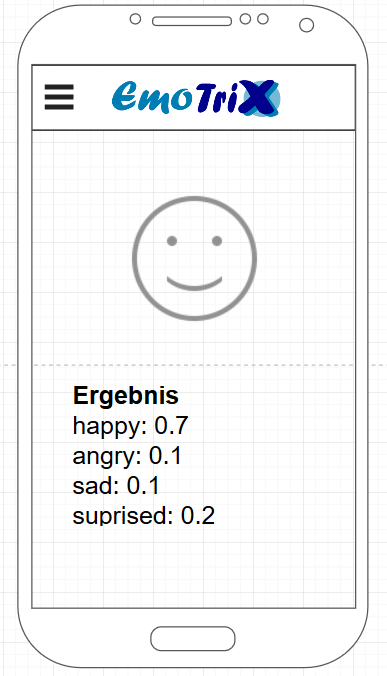
\includegraphics[width=10cm]{Bilder/Mockup-Gesichtserkennung.png}
	\label{img:Mockup-Gesichtserkennung}
	\caption[Mockup - Gesichtserkennung vor Senden des Bilds(links) und Testergebnis(rechts)]{Mockup - Gesichtserkennung vor Senden des Bilds(links) und Testergebnis(rechts)}
\end{figure}
Während der Analyse soll dem Nutzer durch einen Ladebalken signalisiert werden, dass die Daten gerade verarbeitet werden. Auf der Ergebnisseite soll neben dem analysierten Bild das Ergebnis angezeigt werden und außerdem die Möglichkeit bestehen ein neues Bild zu machen oder das gleiche Bild erneut zu analysieren.
\subsubsection{Auswertung}
\subsubsectionauthor{Torben Brenner}
Durch betätigen des Auswertungkopfes auf der Startseite der Anwendung, sollen die bisher erfassten Daten analysiert werden. Das Ergebnis dieser Analyse soll dem Nutzer auf der Auswertungsseite dargestellt werden. Diese besteht aus einem Kreisdiagramm und einem Zeitstrahl.
\begin{figure}[h]
	\centering
	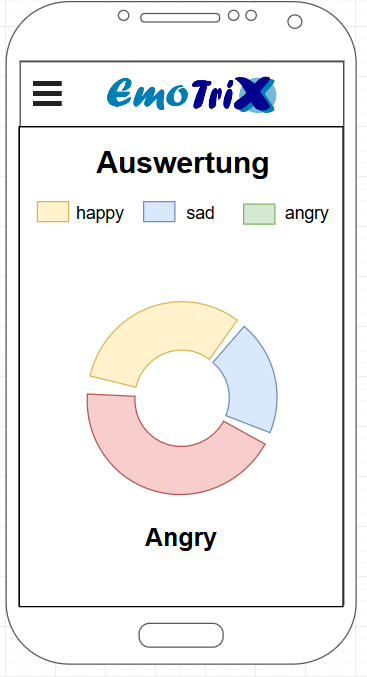
\includegraphics[width=10cm]{Bilder/Mockup-Auswertung.png}
	\label{img:Mockup-Auswertung}
	\caption[Mockup - Auswertung]{Mockup - Auswertung}
\end{figure} \newline
Die Farben des Kreisdiagramms werden durch eine Legende erklärt, d.h. sie werden den einzelnen Emotionen zugeordnet. Durch berühren einer Farbe soll der Nutzer den konkreten Wert für die Emotion angezeigt bekommen. Unter dem Kreisdiagramm soll außerdem ein Zeitstrahl angezeigt werden. Da es später möglich sein soll, Daten im Hintergrund zu erfassen ist es deutlich sinnvoller, die erfassten Daten nicht alle auf einmal zusammen zu rechnen, sondern den Nutzer einen Bestimmten Zeitpunkt auswählen zu lassen. Mit Hilfe des Zeitstrahls soll der Nutzer diese Möglichkeit geboten bekommen.
\newpage
\section{Umsetzung des Prototypen emoTrix}
In diesem Abschnitt wird die Umsetzung des Prototyps beschrieben. Dabei werden neben dem Programmcode auch aufgetretene Probleme beschrieben.
\subsection{Umsetzung der Backendlogik}
\subsubsection{Sensor-Klasse}
\subsubsectionauthor{Torben Brenner}
Wie im Konzept beschrieben besteht das Backend der Anwendung aus den Klassen \textit{Decider, CausalityRule} und der Abstrakten Klasse \textit{Sensor}. Im folgenden wird die Umsetzung der einzelnen Klassen beschrieben.\newline
Die Klasse \textit{Sensor} wurde als Abstrakte Klasse umgesetzt. Dies ermöglicht es dem Entwickler, für jeden Test eine Klasse zu implementieren die von der Architektur verstanden wird und in der er die im Test ermittelten Daten auswerten kann. Die Implementation der \textit{Sensor} Klasse sieht folgendermaßen aus: \newline
\begin{lstlisting}[caption={abstrakte Klasse Sensor},language=JavaScript]
export abstract class Sensor{

	observable: Observable<string>;
	sensorObserver: Observer<string>;

	constructor(public decider: Decider){
		this.observable = Observable.create(observer => {
			this.sensorObserver = observer;
		});
	};

	// this forces the specific sensor evaluators to implement this method
	abstract mapper(data: any): IndicatorScore[]; 

	onSensorData(data: any) {
		let indicatorScores = this.mapper(data)
		this.decider.addIndicatorScores(indicatorScores);
	}

}
\end{lstlisting}
Der Konstruktor der Klasse empfängt eine Instanz der Klasse \textit{Decider}, die wie im Konzept beschrieben ein Singleton ist. Die Funktion \textit{onSensorData} wird von den Subklassen aufgerufen, sobald Daten empfangen wurden und stellt die Logik der Sensor Klasse dar. Zuerst wird bei Empfang der Daten, das von erbenden Klassen definierte \textit{Mapping} auf die Daten ausgeführt. Danach werden die Daten dem \textit{Decider} hinzugefügt, welcher diese dann im späteren Verlauf verarbeiten kann(Vgl. \ref{img:Ablauf Erstellung Indicatorscores}). Durch das Schlüsselwort \textit{abstract} wird bei der Funktion \textit{mapper} gekennzeichnet, dass dieser von den erbenden Klassen implementiert werden soll. Die Abstrakte Klasse definiert in diesem Fall nur, dass der Mapper aus den Daten des Sensors eine Liste von \textit{IndicatorScores} erzeugen muss. Ein \textit{IndicatorScores} besteht dabei aus einem \textit{indicator} und einem \textit{score}. Der Score ist als nummerischer Wert definiert und für die Indicator wurde ein eigener Typ definiert. Dieser Typ ermöglicht es, eine einfache Prüfung der Werte gegenüber dem Typ String und bestimmten Werten durchzuführen. Erlaubte Werte für den Typ Indicator sind zum Beispiel: \textit{``stress''} oder \textit{``angryIndicator''}.\newline
Wie im Konzept beschrieben, verwaltet die Klasse \textit{Decider} alle \textit{IndicatorScores}. Um sicherzustellen, dass die Daten nach Zeitpunkt sortiert gespeichert werden, ermittelt die Methode \textit{addIndicatorScores} erst einen Zeitpunkt und speichert danach die Daten in einer List von Objekten, welche den Zeitpunkt und die dazu gehörige Liste von \textit{IndicatorScores} enthalten. Dadurch können Sensoren die \textit{IndicatorScores} einfach dieser Liste hinzufügen, ohne Gefahr zu laufen, sich gegenseitig zu überschreiben.\newline
Um eine Kommunikation der speziellen Sensoren mit den implementierenden Seiten zu erlauben, wurde der Sensor Klasse ein \textit{Observable} hinzugefügt. Dieses ermöglicht es der Seite sich als \textit{Subscriber} einzutragen. Ein \textit{Subscriber} erhält jedes mal eine Mitteilung, wenn die \textit{next} Funktion des Observers aufgerufen wird. Der Observer wird im Konstruktor aus dem \textit{Observable} erzeugt. Subscriber müssen eine Methode implementieren, in der Sie die Nachrichten des \textit{Observable} verarbeiten. Diese Kommunikation ist Beispielsweise in der Implementation des \textit{FaceSensor} zu sehen.
\subsubsection{CausalityRule-Klasse}
\subsubsectionauthor{Torben Brenner}
Um die Auswertung der Daten zu ermöglichen, greift die Klasse \textit{Decider} außerdem auf eine Liste von Kausalitätsregeln zu. Diese können mit der Klasse \textit{CausalityRule} definiert werden.
Der Konstruktor dieser Klasse nimmt zwei Parameter entgegen. Der Parameter \textit{condition} repräsentiert eine Bedingung, welche eintreten muss sodass die Kausalitätsregel angewandt wird. Die Bedingung wurde innerhalb der Anwendung durch einen Typ umgesetzt. Der Typ prüft dabei auf eine Funktion, die entweder einen oder zwei \textit{indicator} als Parameter entgegennimmt, und als Rückgabewert wahr oder falsch zurückgibt.\newline
\begin{lstlisting}[caption={Typ condition}, language=JavaScript]
	type Condition = (indicatorA: IndicatorScore, indicatorB?: IndicatorScore) => boolean;
\end{lstlisting}
Das bedeutet, dass die Bedingung vom Entwickler frei über die \textit{IndicatorScores} definiert werden kann. Der zweite Parameter der Anwendung repräsentiert die Auswirkungen der Kausalitätsregel beim eintreffen der Bedingung. Um diesen Parameter zu definieren wurde ebenfalls ein neuer Typ angelegt. Dieser prüft auf Funktionen, die sowohl eine Liste von \textit{EmotionScores} als auch eine Liste von \textit{IndicatorScores} entgegen nehmen. Außerdem müssen diese Funktionen eine Liste von \textit{EmotionScores} zurückgeben. Das bedeutet, dass in Funktionen dieser Art irgendeine Manipulation der \textit{EmotionScores} stattfinden muss. Die \textit{IndicatorScores} werden benötigt, um eine Veränderung der \textit{EmotionScores} abhängig von ihnen zu ermöglichen. Der zweite Parameter der Kausalitätsregel ist eine Liste solcher Funktionen. Mit diesen beiden Funktionen kann nun in der Klasse \textit{CausalityRule} eine neue Funktion definiert werden, die prüft ob eine Bedingung eingetroffen ist und in diesem Fall, alle Auswirkungen der Regel ausführt. \newline
\begin{lstlisting}[caption={execute Funktion der Klasse CausalityRule},language=JavaScript]

public execute(data : Array<EmotionScore>, indicatorScores: IndicatorScore[]) {
	indicatorScores.forEach((indicatorScore) =>{
		if(this.condition(indicatorScore)){
			this.effects.forEach((effect) => {
				data = effect(data);
			})
		}});
		return data;
	}
}

\end{lstlisting}
Diese Funktion kann nun von der Klasse \textit{Decider} ausgeführt werden.
\subsubsection{Decider-Klasse}
\subsubsectionauthor{Lukas Seemann}
Im folgenden Abschnitt wird die Implementierung der wichtigsten Funktionen der \textit{Decider} Klasse aufgezeigt und beschrieben. \newline
\begin{lstlisting}[caption={Atrribute der Decider-Klasse}, language=JavaScript]
@Injectable()
export class Decider {

data: Array<{timestamp: number, indicatorScores: IndicatorScore[]}> = [];
resultData: Array<{timestamp: number, emotionScores: EmotionScore[]}> = [];
causalityRules: Array<CausalityRule> = CRarray;

	...
}
\end{lstlisting}
In Listing ? sind die Attribute der \textit{Decider}-Klasse, wie sie auch schon in der Architektur eingeführt worden abgebildet. Das Array \textit{data} in Zeile 4 enthält IndicatorScores mit dem Zeitpunkt in Millisekunden, an dem diese Scores hinzugefügt wurden. Das Hinzufügen ist über die Mapper der einzelnen Sensoren geschehen, die die addIndicatorScore-Funktion des Deciders aufrufen.\newline
In Zeile 5 wird das \textit{resultData}-Array initialisiert. Anhand der vorhandenen IndicatorScores im \textit{data}-Array werden mithilfe der Kausalitätsregeln für alle 10 Sekunden in EmotionScores umgewandelt. Wie dies umgesetzt ist, ist in der decide-Funktion zu sehen. \newline
In Zeile 6 wird das Array der \textit{CausalityRules} über eine Konstante \textit{CRArray} initialisiert. Dieses konstante Array wird in Kapitel 4.3.2 genauer beschrieben. \newline \newline
\begin{lstlisting}[caption={decide-Funktion der Decider-Klasse}, language=JavaScript]
public decide(){
	let start: number = this.findRange().start;
	let end: number = this.findRange().end;
	for(var i:number = start; i<=end; i= i+ 10000){
		var j: number = i + 9999;
		this.assumeEmotion(i, j);
	} 
}
\end{lstlisting}
Die decide-Funktion ist in Listing 5 abgebildet. Mithilfe der internen findRange-Funktionen werden in den Zeilen 2 und 3 die minimale beziehungsweise maximale \textit{timestamp} des \textit{data}-Array bestimmt. So hat man der ersten und letzten Zeitpunkt (in Millisekunden) gefunden, zu dem IndicatorScores durch die einzelnen Test hinzugefügt wurden. \newline
Mithilfe einer for-Schleife (Zeile 4) wird anschließend in 10 Sekunden-Schritten über den durch \textit{start} und \textit{end} festgelegten Bereich iteriert. Dabei wird in der for-Schleife in Zeile eine Hilfsvariable \textit{j} eingeführt, die mit dem Iterator \textit{i} plus 9999 Millisekunden initialisiert wird. Mithilfe von \textit{i} und \textit{j} wird also in jedem Iterationschritt ein Intervall von 10 Sekunden festgelegt. Auf dieses Intervall wird in Zeile 6 die assumeEmotion-Funktion angewendet. \newline
\begin{lstlisting}[caption={assumeEmotion-Funktion der Decider-Klasse}, language=JavaScript]
private assumeEmotion(start: number, end: number){
	let currentIndicators = this.data.filter(e => e.timestamp >= start &&   e.timestamp <= end)
	var emotionScores: Array<EmotionScore> = this.executeCausalityRules(currentIndicators);
	this.resultData.push({ timestamp: start, emotionScores: emotionScores});
}
\end{lstlisting}
Listing 6 zeigt den Aufbau der assumeEmotion-Funktion, die einen \textit{start} und ein \textit{end} als Parameter erhält. Anhand dieser Zahlen wird anfangs in Zeile 2 das \textit{data}-Array gefiltert. Hierbei werden alle Einträge in eine Variable \textit{currentIndicators} geschrieben, die mit ihrer \textit{timestamp} zwischen \textit{start} und \textit{end} liegen. \newline
In Zeile 3 wird dann eine neue Variable \textit{emotionScores} intialisiert, die als Wert das Ergebnis der executeCausalityRules-Funktion angewandt auf die \textit{currentIndicators} erhält. Die Implementierung dieser Funktion, die EmotionScores zurückliefert, ist in Listing 7 zu sehen. In Zeile 4 von Listing 6 werden dann diese Emotionscores mit der \textit{start}-Timestamp zum \textit{resultData}-Array hinzugefügt. \newline 
\begin{lstlisting}[caption={executeCausalityRules-Funktion der Decider-Klasse}, language=JavaScript]
private executeCausalityRules(data: Array<{timestamp: number, indicatorScores: IndicatorScore[]}>){   
	var emotionScores: EmotionScore[] = [];
	emotions.forEach(emotion => {
		var emotionScore : EmotionScore = {emotion, score: 0};
		emotionScores.push(emotionScore);
	});
	data.forEach((e) =>  { 
		this.causalityRules.forEach((causalityRule) => {
			emotionScores = causalityRule.execute(emotionScores, e.indicatorScores)  ;
		})}
	)
	return emotionScores;
}
\end{lstlisting}
Die executeCausalityRules-Funktion erhält als Input ein Array von \textit{timestamp}-\textit{IndicatorScores}-Kombinationen. Zunächst wird in Zeile 2 ein leeres EmotionScore-Array initialisiert. In den Zeilen 3 bis 6 wird dieses dann befüllt, indem für jede vorhandene Emotion (angry, happy, sad, suprised) ein Score von 0 angelegt wird. So erhält man EmotionScores, wobei jede Emotion mit 0 bewertet ist. \newline
Im Anschluss daran wird in Zeile 7 über jeden vorhandenen Eintrag des Input itereriert. Für jeden Eintrag, der aus \textit{timestamp} und \textit{indicatorScores} besteht, wird dann jede im konstansten CausalityRules-Array enthaltene Kausalitätsregel ausgeführt (Zeile 8 bis 10). Durch jede ausgeführte Kausalitätregel werdne die ursprünglich initialisierten EmotionScores modifiziert. Dies wird für alle Einträge im Input der Methode wiederholt. Am Ende werden die final modifizierten EmotionScores zurückgegeben (Zeile 12). 
\subsection{Datenerfassung in Form von Emotionstests}
\subsubsection{GSR-Test}
\subsubsectionauthor{Lukas Seemann}
Die Erfassungsmöglichkeit mit der höchsten Priorität war die Messung der Hautleitfähigkeit mithilfe von EDA- beziehungsweise GSR-Sensoren. Da dies nicht mit im Smartphone enthaltenen Sensoren möglich war, wurde zusätzlich ein Arduino-Mikrocontroller benötigt, um die Messung durchzuführen. Zunächst wird die Entwicklung auf dem Arduino-Board mit allen zusätzlichen Modulen beschrieben. Im Anschluss daran wird thematisiert, wie das Arduino-Board mit der App verbunden wurde. \newline
Für das Projekt wurde ein Arduino UNO R3 Board verwendet. \footcite[Vgl.][]{Ard18} Dieser kann mit Stromzufuhr über ein Netzteil oder per USB betrieben werden. Als Sensor wurde ein GSR Sensor des Grove-Toolkits verwendet\footcite[Vgl.][]{Gro18}, der bereits in Abbildung 5 gezeigt wird. Am Sensor selbst werden die Elektroden für die Finger angebracht. Da ein handelsübliches Arduino UNO R3 Board nicht über den benötigten Anschluss für den Grove GSR-Sensor verfügt, muss zusätzlich noch ein Grove Base Shield angebracht werden. Dieses kann auf das Arduino Board aufgesteckt werden und erweitert es um viele verschiedene Anschlüsse, unter anderem für Sensoren.
\begin{figure}[h]
	\centering
	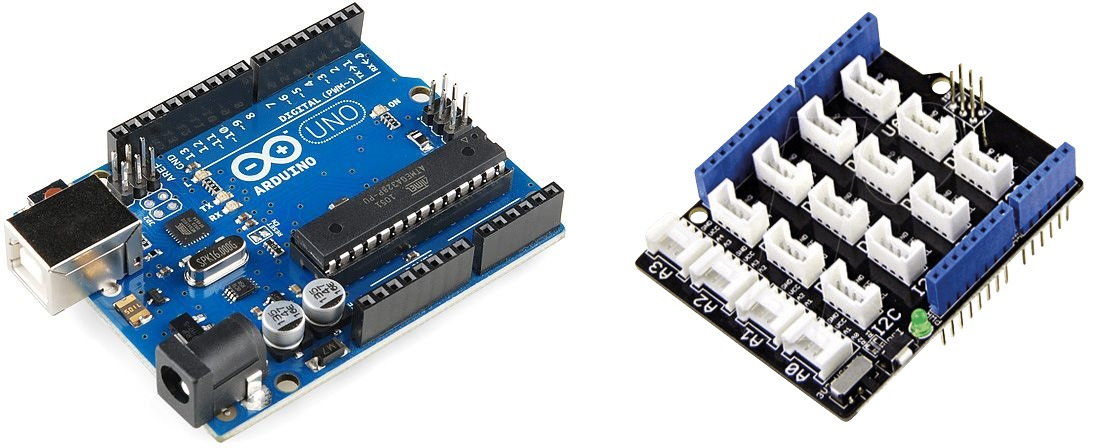
\includegraphics[width=16cm]{Bilder/arduino.jpg}
	\caption[Arduino UNO R3 (links) und Grove Base Shield]{Arduino UNO R3 (links) und Grove Base Shield\footnotemark}
\end{figure}%
\footcitetext[Bilder von:][]{Sou18, Rei18}
\newline \newline
Mit diesen Komponenten werden die vom Sensor zurückgelieferten Daten an den Arduino geleitet. Von dort aus müssen die Daten, an die mobile Applikation weitergeleitet werden. Aus diesem Grund muss an das Arduino Board ein Bluetooth-Modul angebracht werden, das Daten senden und empfangen kann. Das Empfangen von Daten ist notwendig, um die Messung zu Starten, wohingegen das Senden für die Übermittlung der Sensordaten benötigt wird. Heutige Smartphones verfügen meistens immer über eine Bluetooth-Schnittstelle, aus welchem Grund Bluetooth gut für die Übertragung geeignet ist. Eine weitere Möglichkeit wäre die Übertragung über WiFi gewesen. Das Arduino-Board wurde mit einem HC05-Bluetooth-Modul erweitert, welches Daten senden und empfangen kann. Dieses ist in Abbildung ? zu sehen.
\begin{figure}[h]
	\centering
	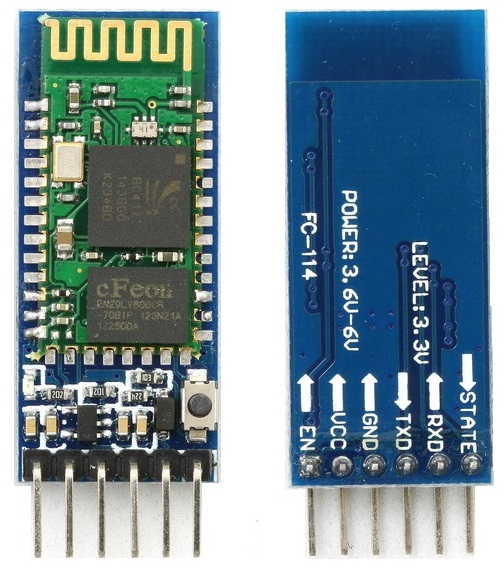
\includegraphics[width=7cm]{Bilder/hc05.jpg}
	\caption[HC-05-Bluetooth-Modul für Arduino]{HC-05-Bluetooth-Modul für Arduino\footnotemark}
\end{figure}%
\newline
Die Beschreibung der Entwicklungsarbeiten wird in zwei Teile aufgespalten. Der erste Teil ist der Quellcode des Arduinos, der zweite Teil die Entwicklung des Emotionstest in der emoTrix-App. \newline
In Listing ? ist der Quellcode des Arduinos abgebildet. In Zeile 1 wird die SofwareSerial-Bibliothek eingebunden, die eine Verwendung der Pins des Arduinos für verschiedene Module ermöglicht. In Zeile 2 wird dem Arduino mitgeteilt, dass auf den Pins 10 und 11 ein Bluetooth-Modul angeschlossen ist und eine Konstante (GSR) festgelegt, die auf den Anschluss A0 des Grove Shields verweist, an dem der GSR Sensor angeschlossen ist. \newline
Generell besteht der Programmcode des Arduinos immer aus zwei Bestandteilen: einem Setup-Block und einem Loop-Block. Der Setup-Block wird einmalig beim Einschalten des Arduinos ausgeführt. Danach wird der Loop-Block solange wiederholt, bis der Arduino ausgeschalten wird. \newline
In Zeile 7 innerhalb des Setup-Blocks wird die Geschwindigkeit der seriellen Datenübertragung der Ports des Arduinos, die mit dem Bluetooth-Modul verbunden sind. Hierbei wird die Geschwindigkeit auf 9600 Bits pro Sekunde gesetzt.\footcite[Vgl.][]{Ard18b} Dies entspricht der üblich verwendeten Geschwindigkeit und hat in Tests sehr gut funktioniert. \newline
\begin{lstlisting}[caption={Quellcode des Arduinos},style=Arduino]
#include <SoftwareSerial.h>
SoftwareSerial BTserial (10, 11); const int GSR=A0;
int sensorValue=0; int gsr_average=0;
boolean measuring = false; char BTString;

void setup(){
	BTserial.begin(9600);
}

void loop(){
	BTString = BTserial.read();
	if(BTString == 'S'){
		measuring = true;
	}
	if(BTString == 'F'){
		measuring = false;
	}
	if(measuring){
		long sum=0;
		for(int i=0;i<10;i++){ 
			sensorValue=analogRead(GSR);
			sum += sensorValue; delay(5);
		}
		gsr_average = sum/10;
		BTserial.print(gsr_average); BTserial.println( ";");
	}
}
\end{lstlisting}
Der Loop-Block beginnt in Zeile 11 mit dem Auslesen der Daten, die über das Bluetooth-Modul empfangen werden. Die Variable \textit{BTString} wird mit diesen Daten beschrieben. Die App muss zum Starten der App den String \textit{S} (für Start) per Bluetooth übertragen. Ist dies der Fall, wird die Variable \textit{measuring} auf true gesetzt. Mit dem String \textit{F} (für Finished) kann die App dem Arduino das Stopsignal für die Messung geben. Demenstprechend wird \textit{measuring} auf false gesetzt. Dies ist in den Zeilen 15 bis 17 umgesetzt. \newline
In Zeile 18 wird über die \textit{measuring}-Variable überprüft, ob gemessen werden soll. Wenn ja, wird eine Variable für die Summe von 10 Messdaten initialisiert. Anschließend werden in Abstand von 5 Millisekunden 10 Messungen durchgeführt. In Zeile 21 wird die eigentliche Messung des Sensors durchgeführt. Der hier verwendete GSR-Sensor liefert als Output einen Integer-Wert, der die Stromspannung auf dem seriellen Port des Arduinos in Volt entspricht. Dieser Wert hängt von der gemessenen Hautleitfähigkeit ab. Die Umrechnung in den Hautleitfähigkeit geschieht dann in der App und wird im Anschluss noch betrieben. Im Arduino-Code selbst werden die Daten überliefert, die auch der Sensor übermittelt. Alle 10 Messungen werden nach und nach aufaddiert. Dies geschieht in der for-Schleife in den Zeilen 20 bis 23. Anschließend wird die Summe durch 10 geteilt, sodass man den Durchschnitt aller 10 Werte erhält. Dieses Verfahren wird durchgeführt, da die Messdaten des Sensors Schwankungen aufweisen, die dadurch eliminiert werden können. In Zeile 25 wird schließlich der Messwert auf den Port des Bluetooth-Moduls geschickt und damit versendet. Als Trennzeichen zum nächsten Wert wird ein Semikolon angehängt. \newline
Wenn die Messung gestartet wurde, erhält die mobile Applikation also alle 50 Millisekunden vom Arduino per Bluetooth einen Integer-Wert übermittelt. \newline
Die Daten, die der Arduino schickt, müssen innerhalb der App verarbeitet werden. Hierfür wurde eine neue TestPage mit dem Namen GSRPage erstellt. Diese Page dient dazu, sich mit dem Arduino Bluetooth-Modul zu verbinden und die Messung zu starten und zu stoppen. Zusätzlich werden die gemessenen Werte in einem Graphen dargestellt, um zu veranschaulichen, wie sich die Hautleitfähigkeit während der Messung ändert. \newline \newline
In der gsr.ts-Datei sind alle Funktionen hinterlegt, die alle Methoden für die Umsetzug der genannte Funktionalitäten implementiert. In Listing 2 ist ein Ausschnitt aus der Typescript-Datei mit den wichtigsten Funktionen abgebildet. \newline
\begin{lstlisting}[caption={JS Code}, language=JavaScript]
startMeasuring(){
this.bluetoothSerial.write('S').then((data: any) => { })
.catch((e) => {
console.log(e);
});;
}

stopMeasuring(){
this.bluetoothSerial.write('F').then((data: any) => {})
.catch((e) => {
console.log(e);
});
}
\end{lstlisting}
Die Funktion \textit{startMeasuring} implementiert das Starten der Messung. Für die GSRPage wurde das Ionic-Package Bluetooth Serial hinzugefügt, das Bluetooth-Optionen des Smartphones für die App verfügbar macht. Das Package wird hier mit \textit{this.bluetoothSerial} referenziert. Das Pairen und Verbinden des Smartphones mit dem Bluetooth-Modul ist selbsterklärend (über eine \textit{connect}-Methode) und deswegen im Listing nicht aufgeführt. Nachdem die Verbindung eingerichtet wurde, kann die \textit{startMeasuring}-Funktion aufgerufen werden. Dabei wird in Zeile 2 mit \textit{write} ein String an das verbundene Bluetooth-Modul gesendet. Wie bereits beschrieben muss zum Start der String \textit{S} gesendet werden. Falls ein Fehler auftritt, wird dieser in Zeile 4 geloggt. Wenn alles ordnungsgemäß funktioniert, empfängt der Arduino den String und startet anschließend die Messung.\newline
Die \textit{stopMeasuring}-Funktion funktioniert analog zur \textit{startMeasuring}-Funktion mit dem Unterschied, dass hier der String \textit{F} zum Stoppen der Messung gesendet wird.
\newline
\begin{lstlisting}[caption={JS Code}, language=JavaScript]
this.bluetoothSerial.subscribe(";").subscribe(function (data){
		self.value = data.substring(0,data.length - 1);
		self.value = ((1024+2*self.value)*10000)/(512-self.value);
		if(self.time%5 == 0){
			if(self.time != 0){
				var data: any = {value: self.value, oldValue: self.oldValue};
				self.GsrSensor.onSensorData(data);
			}
			self.oldValue = self.value;
		} 
		if(self.time%20 == 0){
			self.addData(self.lineChart,self.time, self.value); 
		}
		self.time++;
	}, function (error){
		console.log(error);
});
\end{lstlisting}
In Listing 6 ist implementiert, dass das Bluetooth des Smartphones auf einen neu eintreffenden Integer-Wert des Arduinos reagieren kann. Das BluetoothSerial dient dabei als Observable, den die App abonnieren kann. Dies bedeutet, dass die App darauf hingewiesen wird, wenn neue Daten angekommen sind. Mit \textit{subscribe(";")} wird die App jedes Mal informiert, wenn ein Semikolon übertragen wurde. Das Semikolon wurde im Arduino-Code als Trennzeichen eingesetzt und signalisiert, dass ein Integer-Wert abgeschlossen ist. Mit dem nächsten \textit{subscribe} wird bestimmt, was ausgeführt wird, wenn ein Semikolon empfangen wird. Als \textit{data} (Zeile 1, Ende) wird immer alles übertragen, was seit dem letzten Ausführen der Funktion übertragen wurde. Es handelt sich also immer um einen Integer-Wert und das Semikolon. In Zeile 2 wird aus diesem Grund das letzte Zeichen der Übertragung abgeschnitten, sodass der \textit{value}-Variable nur der Integer-Wert zugewiesen wird.
In Zeile 3 folgt die Umwandlung des Integer-Wert, der der Stromspannung auf dem seriellen Port entspricht, in den Hautwiderstand. \newline Nach Herstellerangaben kann mit der Formel \textit{(1024+2*x)*10000)/(512-x)} der Hautwiderstand berechnet werden, wobei x der gemessenen Stromspannung entspricht.\footcite[Vgl.][]{Gro18} Warum diese Formel genau so aussieht, hat mit dem internen Aufbau des Sensors zu tun, der aus Analog-Digital-Umsetzern und Verstärker aufgebaut ist. \footcite[Vgl.][1. Forumsantwort]{Com18} Da die genaue Erklärung der Formel sehr komplex ist und den Rahmen der Arbeit sprengen würde, wird die Formel hier nicht weiter thematisiert. Wichtig ist, dass man durch diese Umrechnung man den Hautwiderstand des Benutzers in Ohm erhält. \newline
Da alle 50 Millisekunden ein Wert übertragen wird, wird kein neuer Timer benötigt. Dieser wurde anfangs mit dem Wert 0 initialisiert und in Zeile 14 nach jedem neuen Wert um 1 erhöht. Da ein Wert und damit eine Verabeitung alle 50ms für die App einen sehr hohen Workload bedeutet würde, wird nur jeder fünfte übertragene Wert betrachtet. Dies ist in Zeil 4 mit einer if-Bedingung umgesetzt. In Zeile 6 werden immer zwei aufeinander folgende Ohm-Werte zusammengefasst und anschließend in Zeile 7 die onSensorData-Methode mit diesen Daten aufgerufen. Zwei Werte sind für den Mapper trivialerweise genug, um zu schauen ob der Wert gestiegen oder gesunken ist. Da am Anfang nur der erste Wert vorhanden ist, wird dieser Fall in Zeile 5 abgefangen. Das Setzen des alten Werts (\textit{oldValue}) geschieht in Zeile 9. \newline
In Zeile 11 bis 13 wird implementiert, das außerdem jeder zwanzigste Wert in einem Graphen auf der GUI eingetragen wird. Einer häufigere Darstellung ist ebenfalls nicht sehr vorteilhaft für die Benutzung der App, da dies sehr rechenlastig ist. Der Trend des Graphen ändert sich außerdem nicht wesentlich, wenn nicht alle Datenpunkte eingetragen werden. \newline
In Zeile 15 bis 17 wird letzlich noch das Error-Handling implementiert.
\subsubsection{Face-Test}
\subsubsectionauthor{Torben Brenner}
Eine der am höchsten priorisierten Erfassungsmöglichkeiten für Emotionen, war die Messung der Emotionen anhand der Mimik des Menschen mithilfe der Smartphonekamera. Wie im Mockup\footnote{siehe \ref{section:Mockup-Gesichtserkennung} S.\pageref{section:Mockup-Gesichtserkennung}} beschrieben soll der Nutzer zuerst ein Bild machen können und sich dieses anzeigen lassen können, bevor es ausgewertet werden soll. Wenn das Bild zur Analyse freigeben wird, soll dem Nutzer ein Ladebildschirm angezeigt werden. Die Analyse selbst wird nicht auf dem Smartphone durchgeführt, sondern mit Hilfe der Gesichtserkennungsschnittstelle von Microsoft\footcite[siehe ][]{Mic18}.\newline
Zu Beginn der Entwicklung wurde eine Komponente entwickelt, welche das Schießen eines Fotos ermöglicht. Ionic-Komponenten bestehen aus einem HTML-Template, einer SCSS Datei und einem TypeScript Script. Diese Aufteilung in drei Dateien ermöglicht eine Trennung von grafischer Darstellung und der Logik. Die grafische Darstellung der Komponente besteht aus einem Bild, dass nur angezeigt wird wenn mit der Komponente auch ein Bild gemacht wurde, und einem \textit{Ionic-Button}, der das Fotografieren auslöst. Interessanter ist die Logik der Komponente, die daraus besteht abhängig von der der Auswahl des Entwicklers entweder ein Bild zu machen oder eine Videoaufnahme zu starten. Dies wird mit der Übergabe eines Input Parameters ermöglicht.
\begin{lstlisting}[caption={Input und Output der Kamera Komponente}, language=JavaScript]
	@Input() pictureMode: boolean;
	@Output() sourceChanged: EventEmitter<String> = new EventEmitter<String>();
\end{lstlisting}
Da die Komponente aber auch die Bilder, die mit ihr gemacht wurden, herausgeben soll wird ein \textit{Output} definiert. Dieser wird mit Hilfe eines EventEmitters realisiert, der ein Event auslöst auf das andere Teile der Anwendung, die eine Kamera Komponente implementieren reagieren können. Das Event gibt hierbei einen String aus, der in diesem Test dem Base64 codierten Bild entspricht. Im folgenden zusehen ist die Einbindung der Kamera Komponente in den Face-Test. \newline
\begin{lstlisting}[caption={Einbindung Kamera Komponente}, language=HTML]
	<camera [pictureMode]="true" (sourceChanged)="onSourceChanged($event)"></camera>
\end{lstlisting}
Das Fotografieren wird in Ionic mit Hilfe einer \textit{native} Komponente umgesetzt. Diese Komponente erlaubt den plattformunabhängigen Zugriff auf die Kamera\footcite{Ion18e}. Dazu wird in der App direkt eine Weiterleitung an die ausgewählte Kamera App des Nutzers durchgeführt. Nachdem der Nutzer mit dieser ein Bild gemacht hat, kann entweder der Speicherort oder das Bild selbst zurückgegeben werden. Der zurückgegebene Wert wird dann von der Kamera Komponente per \textit{EventEmitter} ausgegeben.\newline
Wie in der Einbindung der Komponente zu sehen ist, wird beim auslösen des Events \textit{sourceChanged} im Face-Test eine Funktion aufgerufen. Dies geschieht mittels \textit{Event Binding}. Die aufgerufene Funktion speichert den empfangenen Source Wert in einer lokalen Variable im Face-Test. Bei Betätigung des \textit{Send Picture Buttons} wird daraufhin die Analyse gestartet. Die Analyse wird von der \textit{FaceSensor} Klasse durchgeführt. Dazu wird vom Face-Test die Funktion \textit{prepareData} aufgerufen, die eine HTTP POST Anfrage an die Microsoft Gesichtserkennungsschnittstelle durchführt. Die Details der Anfrage sind in folgender Codeausschnitt zu sehen:
\begin{lstlisting}[caption={Aufbau Anfrage an Gesichtserkennungsschnittstelle}, language=JavaScript]
{
	url: 'https://westeurope.api.cognitive.microsoft.com/face/v1.0/detect?returnFaceAttributes=emotion',
	type: 'POST',
	processData: false,
	headers: {
		'Ocp-Apim-Subscription-Key': '{Api Key}'
	},
	contentType: 'application/octet-stream',
	data: this.makeblob(base64Data)
}
\end{lstlisting}
Das einzig nennenswerte an dieser Anfrage ist die Übertragung des Base64 codierten Bildes. Diese geschieht nämlich in Form eines Blob(Binary Large Object). Laut \textit{MDN web docs} ist ein Blob eine ``dateiähnliche Menge unveränderlicher Roh-Daten''\footcite[Vgl. ][Abschnitt Übersicht]{Mdn18}. Diese wird nicht nur bei der Übertragung großer Datenmengen verwendet, sondern auch beim Abspeichern größerer Dateien in Datenbanken. Um das Base64 codierte Bild in einen Blob zu übertragen wurde die Hilfsmethode \textit{makeblob} genutzt. Diese wurde nicht von mir selbst entwickelt sondern von Kalpesh Singh\footcite[Vgl. ][Antwort von Kalpesh Singh]{Sin16}. Die Funktion trennt die \textit{ContentType} Informationen von den Roh-Daten und überträgt diese dann in einen neuen Blob. Bei der Base64 Codierung müssen die Roh-Daten erst mit Hilfe der JavaScript Funktion \textit{charCodeAt} in Ganzzahl Werte übertragen werden. Der generierte Blob wird dann im \textit{Body} der HTTP Anfrage mit übertragen.\newline
Nach dem senden der Request wird auf der Oberfläche der App dem Nutzer mit Hilfe eines \textit{Ionic Loaders}\footcite{Ion18f} signalisiert, dass im Hintergrund gerade eine Verarbeitung der Daten stattfindet. Da die Sensor Klasse ein sogenanntes \textit{Observable} implementiert, können Statusmeldungen zwischen der Face-Test Seite und dem \textit{FaceSensor} ausgetauscht werden. Die Statusmeldungen werden auf Seiten des \textit{FaceSensor} initiert und von der Seite mit Hilfe einer \textit{Callback} Funktion verarbeitet.
\begin{lstlisting}[caption={Callback Methode auf FaceSensor Observable}, language=JavaScript]
	this.faceSensor.observable.subscribe(data => {
		if(data == "Sending data to Microsoft"){
			this.loader.present();
		}
		if(data == "empty result"){
			this.loader.dismiss();
			alert("Microsoft Server couldn't recognize your face. Please make sure your face is visible");
		}
		if(data.startsWith("result:")){
			console.log("This is a result");
			this.loader.dismiss();
			let emotions = JSON.parse(data.replace("result:", ""));
			console.log(emotions);
			this.faceSensor.onSensorData(emotions);
		}
		if(data.startsWith("error:")){
			this.loader.dismiss();
			let errorString = data.replace("error:", "");
			alert(errorString);
		}
	});
\end{lstlisting}
Die Daten des \textit{FaceSensor} werden mit Strings übertragen. Durch das Schlüsselwort ``result'' wird gekennzeichnet, das es sich beim Rest des Strings um Ergebnis Daten handelt, die mit der \textit{JSON.parse} Methode in ein JavaScript Objekt übertragen werden können. Durch ``error'' wird gekennzeichnet, dass ein Fehler aufgetreten ist der ausgegeben werden soll. Dies wird mit Hilfe eines \textit{alert} umgesetzt. Es kann außerdem passieren, dass die Microsoft Gesichtserkennungsschnittstelle kein Gesicht erkennt. Das ist in unseren Testläufen insbesondere dann aufgetreten, wenn das Bild um 90 Grad gedreht war. Für diesen Fall haben wir eine eigene Fehlernachricht eingebaut.\newline
Wenn aber alles ohne Fehler abgelaufen ist, erhalten wir vom Microsoft Server ein JSON Objekt der Form:
\begin{lstlisting}[caption={Ergebnis Gesichtserkennungsschnittstelle, Beispiel Microsoft}, language=JavaScript]
[
	{
		"faceId": "579838a9-fb50-4333-8770-32858b2d0fc6",
		"faceRectangle": {
			"top": 131,
			"left": 177,
			"width": 162,
			"height": 162
		},
		"faceAttributes": {
			"emotion": {
				"anger": 0,
				"contempt": 0,
				"disgust": 0,
				"fear": 0,
				"happiness": 0.001,
				"neutral": 0.987,
				"sadness": 0.001,
				"surprise": 0.01
			}
		}
	}
]
\end{lstlisting}
Aus diesem Objekt interessiert uns der Datensatz \textit{emotion}. Diesen kann man mittels JavaScript einfach auslesen. Eine Problematik die derzeit nicht im Face-Test behandelt wird, ist die Verarbeitung von mehreren Gesichtern in einem Bild. In diesem Fall würde ein weiteres Objekt mit einer anderen \textit{faceId} zurückgegeben werden. Für die Zukunft wäre es denkbar die \textit{faceId} in der Ausgabe zu kontrollieren und den Nutzer zur Identifikation ein erstes Bild machen zu lassen in dem die \textit{faceId} ermittelt wird. Dies wäre zum Beispiel in den Settings möglich. Problematisch an diesem Ansatz ist aber, dass die \textit{faceId} nur temporär ist und nach 24 Stunden abläuft. Also müsste der Nutzer nach einem Tag Inaktivität diese neu setzen.\newline
Zum Abschluss des Face-Tests fehlt nur noch die Implementierung der \textit{mapper} Funktion im \textit{FaceSensor}. Diese ist relativ einfach, da der Funktion einfach das \textit{emotion} Objekt aus der HTTP Antwort weitergegeben werden kann. Dort werden die Werte dann in \textit{IndicatorScores} übertragen, was in diesem Fall trivial ist, da Sie bereits Prozente darstellen und somit einfach übernommen werden können. Das senden der Daten an den Decider wird durch die Funktion \textit{onSensorData} der Klasse \textit{Sensor}, von der der \textit{FaceSensor} erbt, bereits übernommen, womit die Implementation abgeschlossen ist.   
\subsection{Beschreibung der implementierten Kausalitätsregeln}
\subsectionauthorlong{Torben Brenner}
Alle von uns implementierten Kausalitätsregeln befinden sich aus Übersichtsgründen in der Datei \textit{CausalityRulesArray.ts}. Hier werden zum aktuellen Zeitpunkt sechs verschiedene Kausalitätsregeln implementiert(zwei davon für den GSR-Test und vier für den Face-Test). Diese Regeln werden zusammen in einem Array exportiert, welches von der \textit{Decider} Klasse eingebunden wird. Im folgenden sollen die verschiedenen Regeln genauer erläutert werden.
\subsubsection{Regeln des GSR-Test}
\subsubsectionauthor{Torben Brenner \& Lukas Seemann}
Da der \textit{Activation} Indikator entweder \textit{0, 0.5 oder 1} sein kann, ist es nur notwendig zwei Regeln für diesen zu implementieren. Wenn der \textit{Activation} Indikator einen Wert von 0.5 hat, ist dieser als neutral anzusehen, d.h. die vom GSR-Sensor erfassten Werte zeigen keine Tendenz für den Stress. In diesem Fall finden keine Veränderungen an den \textit{EmotionScores} statt, weshalb hierfür auch keine Kausalitätsregel zu implementieren ist. Anders sieht das bei den Werten \textit{0 und 1} aus. In diesen Fällen zeigt sich eine Tendenz der erfassten Werte für gestresst(1) oder nicht gestresst(0). Deshalb unterscheidet sich die Bedingung der beiden Regeln gerade mal durch die Prüfung auf den bestimmten \textit{score}. \newline
\begin{lstlisting}[caption={Bedingung der ersten Kausalitätsregel(gestresst)}, language=JavaScript]
	(indicatorScore: IndicatorScore) => {
		return indicatorScore.indicator == <indicator>"activation" && indicatorScore.score == 1;
	}
\end{lstlisting}
Auch die Auswirkungen der beiden Regeln sind sich ähnlich. So werden bei Eintritt der ersten Regel zu den \textit{EmotionScores} für die Emotionen \textit{wütend, fröhlich und überrascht} jeweils eins zu dem Score hinzu addiert. Bei eintritt der zweiten Regel wird stattdessen eins subtrahiert. Diese Änderungen wirken zwar sehr klein im Vergleich zu den Änderungen der Kausalitätsregeln des Face-Test, werden sich aber aufgrund der Menge von Daten in einem Zeitraum dennoch bemerkbar machen. So werden in einer Sekunde circa 20 Werte erfasst, während dem der Face-Test deutlich länger für die Durchführung benötigt.
\subsubsection{Regeln des Face-Test}
\subsubsectionauthor{Torben Brenner}
Für den Face-Test wurden vier Kausalitätsregeln definiert. Von diesen vier Regeln ist jeweils eine für einen bestimmten \textit{EmotionScore}. Da bei der Eignung des Gesichts als Emotionsindiz festgestellt wurde, dass dieses äußert aussagekräftig ist werden die durch den Face-Test erfassten Werte sehr stark gewichtet. Die Werte die vom Test ermittelt werden sind Prozentzahlen, die aussagen wie wahrscheinlich eine bestimmte Emotion ist. Deshalb wird bei der Erfassung eines solchen Wertes dieser mit 100 multipliziert und dann auf den jeweiligen \textit{EmotionScore} addiert. \newline
\begin{lstlisting}[caption={Kausalitätsregel basierend auf Face-Test für Emotion Wut}, language=JavaScript]
	(indicatorScore: IndicatorScore) => {
		return indicatorScore.indicator == <indicator>"angryIndicator" && indicatorScore.score != undefined;    
	},[
		(data: EmotionScore[], indicatorScores :IndicatorScore[]) => {
			let angry = data.find((emotionScore) => {return emotionScore.emotion == <emotion>"angry"});
			let angryIndicator = indicatorScores.find((indicatorScore) => {return indicatorScore.indicator == <indicator>"angryIndicator"});
			angry.score = angry.score + (100 * angryIndicator.score);
			return data;
		}
	]
\end{lstlisting}
Als Bedingung das eine Kausalitätsregel des Face-Test eintritt, ist gewählt das der jeweilige Indikator definiert ist. Diese sind im Normalfall nicht definiert, werden aber bei Erfassung eines Bildes gesetzt. Im Falle der Wut ist der Indikator der sogenannte \textit{angryIndicator}. Bei Eintritt der Bedingung werden die Auswirkungen wie oben beschrieben ausgeführt. Die andern drei Regeln für den Face-Test unterscheiden sich nur durch die Auswahl des \textit{Indicator-} und \textit{EmotionScores}.
\subsection{Benutzeroberfläche der App}
\subsectionauthor{Lukas Seemann}
In diesem Kapitel wird die Benutzeroberfläche der mobilen Applikation beschrieben. Das Kapitel soll auch als Benutzungsanleitung für die einzelnen Funktionen der App dienen.
\subsubsection{HomePage}
\subsubsectionauthor{Lukas Seemann}
In Abbildung ? ist der StartScreen der App zu sehen. Dieser wird aufgerufen, wenn der User die App öffnet. Hier werden dem User alle Emotionstests aufgelistet, die er durchführen kann. Durch ein Klicken auf das Label oder den Pfeil gelangt der User auf den Screen des jeweiligen Tests. Von den aufgelisteten Tests wurde der Keyboard Scanner nicht umgesetzt. Ein Klicken auf dieses Label führt zu einer Meldung, dass die Seite noch nicht implementiert wurde. \newline
Führt der User einen Emotionstest erfolgreich durch, verwandelt sich bei der Rückkehr auf die HomePage der Pfeil am Ende des Test in einen Haken. So erhält der User einen Überblick darüber, welche Test er bereits durchgeführt und welche noch offen sind. \newline
Durch ein Klicken auf den \textit{Auswertung}-Button wird eine Auswertung der Testergebnisse durchgeführt, die zum Zeitpunkt des Klickens im Decider hinterlegt sind. Der User wird anschließend zur DecisionPage navigiert, welche ihm seine Ergebnisse visualisiert. \newline
Über das Klicken der drei Striche in der Toolbar oder ein Swipen nach rechts, wird seitlich ein Menü angezeigt, über welches der User zu weiteren Screens der App gelangen kann. Wie bereits im Mockup beschrieben, gibt es hier die Möglichkeiten auf eine Anleitungsseite, eine Übersicht der durchgeführten Messungen oder eine Einstellungsseite zu gelangen. Aus Zeitgründen konnte hiervon nur die Anleitungsseite umgesetzt werden. Über dieses seitliche Menü kann der User außerdem auch auf jeder beliebigen Seite über die erste Auswahlmöglichkeit (\textit{Home}) zurück zum Startscreen gelangen.
\subsubsection{GSRPage}
\subsubsection{CameraPage}
\subsubsection{DecisionPage}

\newpage
\section{Schluss}
Hier werden wir darauf eingehen was erreicht wurde was nicht und weshalb nicht.
\subsection{Anwendungsszenarien}
\subsectionauthor{Torben Brenner \& Lukas Seemann}
Der im Rahmen dieser Studienarbeit entwickelte Prototyp ist in der Lage, mithilfe der Erfassung von biometrischen Daten auf Emotionen zu schließen. Nun stellt sich die Frage, für welche Anwendungsszenarien die App nützlich sein könnte. Dieser Abschnitt soll diese Frage beantworten. \newline
\subsubsection{Studien}
\subsubsectionauthor{Torben Brenner \& Lukas Seemann}
Die Verwendung von Emotionserkennung über das Smartphone, ermöglicht es sehr einfach neue Studien in diesem Bereich durchzuführen. Durch das verteilen einer einfachen Installationsdatei könnten Studienteilnehmer ohne großen Aufwand an einer Studie teilnehmen. Denkbar wären hierbei Szenarios, bei denen die Teilnehmer zum Beispiel zehn Minuten täglich einen Test durchführen sollen oder in denen Sie durch eine bestimmte Auswahl von Sensoren dauerhaft analysiert werden. Damit wären Studien über den Emotionalen Verlauf eines Arbeitstags möglich.\newline
Unsere Architektur eignet sich insbesondere für solche Fälle, da es möglich ist eine beliebige Anzahl an Sensoren im Hintergrund arbeiten zu lassen und deren Ergebnisse zusammen zu führen. \newline 
Da die Emotion möglichst natürlich sein sollen und nicht bewusst vorgetäuscht beispielsweise durch Grimassen bei der Gesichtserkennung werden sollen, wäre es sinnvoll, die App zu dem Zeitpunkt einzusetzen, wenn die Emotion hervorgerufen wird. Es muss also unmittelbar die erste Reaktion des Anwenders auf Reize von außen eingefangen werden. Hierbei ergibt sich eine mögliche Anwendung der App emoTrix. \newline
Die App kann dazu eingesetzt werden, um zu bestimmen, wie Leute auf verschiedenes Bild- oder Filmmaterial reagieren. Während der Anwender verschiedene Bilder oder Filme zum ersten Mal sieht, müssen verschiedene Emotionstests der App gestartet werden. Am Ende kann man über die Auswertung nachvollziehen, welche Emotion bei welchem Bildmaterial empfunden wurden. Beispielsweise kann der Anwender, während er auf die Bilder reagiert, mit dem GSR-Sensor verbunden sein. Gleichzeitig wird bei jedem neuen Bild direkt bei der Reaktion ein Bild aufgenommen oder bei einem Film zum Beispiel alle 10 Sekunden. Diese Bilder können dann von der App analysiert werden. Zusätzlich kann der Anwender gebeten werden, das Gesehene zu kommentieren. Diese Sprachaufnahmen können auch mit der App analysiert werden. So ist es möglich, eine möglichst genaues Ergebnis der Emotionsbestimmung zu erhalten. \newline
Mithilfe der App kann im Nachhinein eine Studie durchgeführt werden, die untersucht, mit welchen Emotionen Menschen auf Bilder oder Filme reagieren. Hieraus können wertvolle Informationen und Statistiken gewonnen werden, was Menschen generell erfreut, bekümmert oder verärgert. \newline
Im Speziellen könnte auch eine Erweiterung stattfinden, in der Nutzer nicht nur analysiert werden sondern in denen diese dann auch die Auswertung überprüfen. So könnte im Auswertungsbildschirm eine Meldung von falschen Analysen mit eingebaut werden, um kontinuierlich Nutzer Feedback zu sammeln. In einer extrem ausgeweiteten Variante davon, könnte sogar ein neuronales Netz eingesetzt werden, um die Gewichtung von Indizien in Form der Kausalitätsregeln zu verbessern. Dabei würde das Training primär von den Nutzern durchgeführt. 
\subsubsection{Wirtschaft}
Auch in der Wirtschaft ist es interessant, was Kunden während dem Einkauf fühlen. Eine gängige Praxis in Call Centern ist zum Beispiel schon das prüfen des emotionalen Zustandes eines Anrufers. So können die Mitarbeiter im Zweifelsfall direkt deeskalierend mit dem Anrufer/-in sprechen.
\subsubsection{Unterstützung von Autisten}
\subsection{Fazit}
%Archiktektur ist gut, erweiterbar, Viele Anpassungsmöglichkeiten,
%App läuft im Hintergrund
%Kausalitätsregeln hätten besser gemacht werden können
%Wissen bezüglich Emotionsbestimmung hat gefehlt
%Im Prinzip nicht alles in dieser Zeit zu schaffen
\subsection{Ausblick}
\subsectionauthor{Torben Brenner \& Lukas Seemann}
Da von den vorgestellten Erfassungsmöglichkeiten von biometrischen Daten bislang nur die Gesichtserkennung und die Hautleitwiderstand-Messung und damit Platz 1 und Platz 2 der Prioriserungsliste implementiert wurden, kann die App in Zukunft um weitere Emotionstest erweitert werden. Die hier vorgestellten Möglichkeiten können dafür als Vorlage dienen. Der nächste zu implentierende Emotionstest ist die Stimmerkennung. Danach folgt das Analysieren des Tippverhaltens und alternativ können im Anschluss daran auch noch die restlichen Erfassungsmöglichkeiten der Priorsierungsliste als Emotionstest umgesetzt werden. Neue Test können aufgrund der Architektur von emoTrix einfach integriert werden. \newline
Ein Erweiterung der App um Emotionstest führt zu genaueren Ergebnissen, da der Decider so mehr Daten als Entscheidungsgrundlage zur Verfügung hat. Dies ist auf jeden Fall eine wünschenswerte Weiterentwicklung der Anwendung.\newline
Zusärtlich müssen mit der Zeit auch die Kausalitätsregeln verbessert werden. \textbf{TORBEN: schreib was über deine KI Idee ;)} 
% Sollte mit KI Learning verbessert werden können 

\newpage
\addcontentsline{toc}{section}{Literaturverzeichnis}
\printbibliography
\newpage

\section*{Anhänge}
\addcontentsline{toc}{section}{Anhänge}


\end{document}